% TODO: ulepszyć formatowanie - dodać \texttt do nazw funkcji, ujednolicić pi-typy, zrobić aplikację spacjową a nie nawiasową.

\documentclass{beamer}

\usepackage[utf8]{inputenc}
\usepackage{polski}
\usepackage[polish]{babel}
\usepackage{graphicx}

\usetheme{Darmstadt}
\useoutertheme[subsection=false]{miniframes}
\makeatletter
  \beamer@compressfalse
\makeatother

\newcommand{\defn}{:\equiv}

\newcommand{\U}{\mathcal{U}}

\newcommand{\id}{\text{id}}
\newcommand{\comp}{\circ}
\newcommand{\finv}[1]{#1^{-1}}

\newcommand{\refl}[1]{\text{refl}_{#1}}
\newcommand{\inv}[1]{#1^{-1}}
\newcommand{\sq}{\mathbin{\vcenter{\hbox{\rule{.3ex}{.3ex}}}}}

\newcommand{\ap}[2]{\text{ap}_{#1}(#2)}
\newcommand{\apd}[2]{\text{apd}_{#1}(#2)}
\newcommand{\transport}{\text{transport}}

\newcommand{\qinv}{\text{qinv}}
\newcommand{\isequiv}{\text{isequiv}}

\newcommand{\prl}{\text{pr}_1}
\newcommand{\prr}{\text{pr}_2}

\newcommand{\happly}{\text{happly}}
\newcommand{\funext}{\text{funext}}

\newcommand{\idtoeqv}{\text{idtoeqv}}
\newcommand{\ua}{\text{ua}}

\newcommand{\code}{\text{code}}
\newcommand{\encode}{\text{encode}}
\newcommand{\decode}{\text{decode}}

\newcommand{\isContr}{\text{isContr}}
\newcommand{\isProp}{\text{isProp}}
\newcommand{\isSet}{\text{isSet}}
\newcommand{\isGrpd}{\text{isGrpd}}

\newcommand{\Contr}{\text{Contr}}
\newcommand{\Prop}{\text{Prop}}
\newcommand{\Set}{\text{Set}}
\newcommand{\Grpd}{\text{Grpd}}
\newcommand{\Type}{\text{Type}}

\newcommand{\hS}{\mathbb{S}^1}
\newcommand{\base}{\text{base}}
\newcommand{\looop}{\text{loop}}

\newcommand{\I}{\mathbb{I}}
\newcommand{\IZ}{0_\mathbb{I}}
\newcommand{\II}{1_\mathbb{I}}
\newcommand{\seg}{\text{seg}}

\newcommand{\trf}[1]{||#1||}
\newcommand{\tri}[1]{|#1|}

\title{Homotopiczna teoria typów}
\author{Wojciech Kołowski}
\date{14 stycznia 2019}

\begin{document}

\frame{\titlepage}

\addtocontents{toc}{\setcounter{tocdepth}{1}}
\frame{\tableofcontents}

\section{Wstęp}

\begin{frame}{Czym jest HoTT?}
\begin{itemize}
	\item Homotopiczna teoria typów (w skrócie HoTT) to połączenie teorii typów i teorii homotopii.
	\item Jest kolejnym stadium ewolucji teorii typów.
	\item Jest syntetyczną teorią homotopii, dającą nam łatwy dostęp do skomplikowanych pojęć topologicznych.
	\item Jest pomysłem na nowe podstawy matematyki, alternatywne wobec teorii zbiorów.
	\item Jest bardzo potężnym funkcyjnym językiem programowania.
\end{itemize}
\end{frame}

\begin{frame}{Innowacje HoTT}
\begin{itemize}
	\item Homotopiczna interpretacja teorii typów, mocno wspomagająca wyobraźnię zarówno w rozumowaniu, jak i pozwalająca dogłębnie zrozumieć różne detale teorii typów.
	\item Aksjomat uniwalencji $(A \simeq B) \simeq (A = B)$, który głosi, że rzeczy mające tę samą strukturę są identyczne. Rozwiązuje to odwieczny problem nieformalnego utożsamiania poprzez nadużycie języka.
	\item Wyższe typy induktywne, pozwalające w teorii typów:
	\begin{itemize}
		\item Zdefiniować wiele niemożliwych dotychczas obiektów, np. typy ilorazowe albo prezentacje obiektów algebraicznych.
		\item Konstruktywnie rozwiązać wiele problemów, które dotychczas wymagały logiki klasycznej (konstrukcja liczb rzeczywistych Cauchy'ego)
		\item Wyrazić klasyczne pojęcia logiczne (dysjunkcja, kwantyfikator egzystencjalny, aksjomat wyboru) z niemożliwą wcześniej w teorii typów precyzją.
	\end{itemize}
\end{itemize}
\end{frame}

\section{Typy}

\begin{frame}{Teoria typów 1 - podstawy}
\begin{itemize}
	\item Teorię typów w ujęciu HoTTowym można opisać jako system formalny, który za pomocą reguł (osądów) opisuje byty zwane typami. Kluczową innowacją HoTT jest interpretacja typów i wymyślone na jej podstawie aksjomaty rzucające światło na naturę kosmosu.
	\item Reguły dzielą się na ciekawe i nieciekawe.
	\item Nieciekawe to te, które muszą być, żeby wszystko działało, np. do zamieniania kolejności rzeczy w kontekście.
	\item Ciekawe to te, które faktycznie opisują typy. Jest ich pięć rodzajów: reguły formacji, wprowadzania, eliminacji, obliczania i unikalności.
\end{itemize}
\end{frame}

\begin{frame}{Teoria typów 2 - pięć rodzajów reguł}
\begin{itemize}
	\item Reguły formacji mówią, skąd się biorą typy.
	\item Reguły wprowadzania mówią, jak zrobić elementy danego typu.
	\item Reguły eliminacji mówią, jak zrobić coś z elementami danego typu.
	\item Reguły obliczania mówią, jak reguły eliminacji mają się do reguł wprowadzania.
	\item Reguły unikalności mówią, jak reguły wprowadzania mają się do reguł eliminacji.
\end{itemize}
\end{frame}

\begin{frame}{Teoria typów 3 - reguły dla funkcji}

\begin{itemize}
	\item Ćwiczenie: nazwij każdą z reguł (tzn. która to reguła formacji, która obliczania etc.)
\end{itemize}

\begin{center}
	$\displaystyle \frac{\Gamma \vdash A : \U \quad \Gamma \vdash B : \U}{\Gamma \vdash A \to B : \U}$
\end{center}
\begin{center}
	$\displaystyle \frac{\Gamma, x : A \vdash b : B}{\Gamma \vdash \lambda x:A.b : A \to B}$
\end{center}
\begin{center}
	$\displaystyle \frac{\Gamma \vdash f : A \to B \quad \Gamma \vdash x : A}{\Gamma \vdash f\ x : B}$
\end{center}
\begin{center}
	$\displaystyle \frac{\Gamma, x : A \vdash b : B \quad \Gamma \vdash a : A}{\Gamma \vdash (\lambda x:A.b)\ a \equiv b[x := a] : B}$
\end{center}
\begin{center}
	$\displaystyle \frac{\Gamma \vdash f : A \to B}{\Gamma \vdash \lambda x:A.f\ x \equiv f : A \to B}$
\end{center}

\begin{itemize}
	\item Uwaga: w powyższych regułach $\U$ oznacza uniwersum, czyli typ typów, a zatem $\Gamma \vdash A : \U$ oznacza ``$A$ jest typem w kontekście $\Gamma$''.
\end{itemize}

\end{frame}

\begin{frame}{Teoria typów 4 - ciekawostki o regułach}
\begin{itemize}
	\item Każdy typ musi mieć regułę formacji - inaczej nie byłby typem.
	\item Jednak nie każdy typ musi mieć pozostałe reguły.
	\item Typ $\textbf{0}$ nie ma reguły wprowadzania, bo jest pusty i nie ma żadnych elementów.
	\item Uniwersum nie ma reguły eliminacji.
	\item Typ $\textbf{0}$ nie ma także reguły obliczania, co jest oczywiste - nie może jej mieć, skoro nie ma reguły wprowadzania.
	\item Wiele typów, np. sumy i produkty, nie mają reguły unikalności. W zamian za to mają one zdaniową regułę unikalności, tzn. można udowodnić twierdzenie wyglądające dokładnie jak reguła unikalności.
	\item Reguła formacji zawsze jest jedna, bo każdy typ można sformować tylko na jeden sposób. Pozostałych reguł może być więcej. Sumy mają 2 reguły wprowadzania, a produkty 2 reguły eliminacji i wobec tego 2 reguły obliczania.
\end{itemize}
\end{frame}

\begin{frame}{Teoria typów 5 - cztery style definiowania}
\begin{itemize}
	\item Formalnie rzeczy definiujemy za pomocą reguł wprowadzania i eliminacji.
	\item Przykład: funkcję $\text{swap} : \Pi A\ B : \U. A \times B \to B \times A$ możemy zdefiniować jako $\text{swap} \defn \lambda A : \U.\lambda B : \U.\lambda x : A \times B. (\prr(x), \prl(x))$
	\item Zamiast tego często będziemy jednak definiować poprzez dopasowanie do wzorca, jednocześnie pomijając argumenty, które można wywnioskować z kontekstu: $\text{swap}\ (a, b) \defn (b, a)$
	\item Możemy też definiować słownie: niech $\text{swap}$ będzie funkcją, która zamienia miejscami elementy pary. Ten sposób będziemy wykorzystywać do dowodzenia twierdzeń.
	\item Ostatnim stylem jest obrazkowy styl definiowania. Nie jest on używany w książce, ale ja postaram się go wykorzystać podczas tej prezentacji, gdyż dobrze działa na wyobraźnię.
\end{itemize}
\end{frame}

\section{Interpretacja homotopiczna}

\subsection{Część 1}

\begin{frame}{Teoria homotopii 1 - homotopia}
\begin{itemize}
	\item Co to jest homotopia?
	\item Zgodnie z wikipedią, jeżeli $f$ i $g$ są funkcjami ciągłymi z przestrzeni topologicznej $X$ w przestrzeń topologiczną $Y$, to $H : [0; 1] \times X \to Y$ jest homotopią, gdy jest funkcją ciągłą spełniającą $H(0, x) = f(x) \land H(1, x) = g(x)$.
	\item Jeżeli nieco pogmeramy w symbolach, to możemy to zapisać tak: $H: [0; 1] \to (X \to Y)$ jest homotopią, gdy jest ciągła i spełnia $H(0) = f \land H(1) = g$.
	\item Nie przejmuj się, jeżeli definicja cię nie oświeca. Moim zdaniem władowanie jej do nazwy całej teorii jest głupie.
\end{itemize}
\end{frame}

\begin{frame}{Teoria homotopii 2 - ścieżka}
\begin{itemize}
	\item Bardziej podstawowym pojęciem jest ścieżka.
	\item Ścieżka w przestrzeni topologicznej $X$ to funkcja ciągła z $[0; 1]$ w $X$.
	\item Łatwo to sobie wyobrazić: odcinek $[0; 1]$ z pewnością jest ścieżką prowadzącą od $0$ do $1$. Jego obrazem, czyli ścieżką, jest więc pewien ciągły zawijasek, który prowadzi z $f(0)$ do $f(1)$.
	\item Ostatecznie możemy powiedzieć, że homotopia to ścieżka między funkcjami.
	\item Teoria homotopii nie jest jednak teorią ścieżek między funkcjami. Jest to raczej po prostu teoria ścieżek.
\end{itemize}
\end{frame}

\begin{frame}{Teoria homotopii 3 - topologia (algebraiczna)}
\begin{itemize}
	\item Po co to wszystko?
	\item Topologia jest całkiem użyteczna. Ostatnio popularna robi się topologiczna analiza danych. Zamiast prymitywnie przypasowywać do danych proste (regresja liniowa), ludzie próbują lepiej opisywać kształt danych. Topologia bada kształty, więc pasuje jak ulał.
	\item Chcemy więc wiedzieć więcej o topologii, np. czy dwie przestrzenie są takie same czy inne. Tutaj wkracza topologia algebraiczna, czyli dziedzina badająca przestrzenie topologiczne za pomocą metod algebraicznych.
\end{itemize}
\end{frame}

\begin{frame}{Teoria homotopii 4 - grupa podstawowa}
\begin{itemize}
	\item Pętla w punkcie $x$ to ścieżka, która zaczyna się i kończy w punkcie $x$.
	\item Grupa podstawowa przestrzeni $X$ w punkcie $x$ to grupa, której nośnikiem jest zbiór wszystkich pętli w punkcie $x$. Działaniem grupowym jest sklejanie pętli (najpierw pójdź pierwszą pętlą, a potem drugą). Odwrotność to pójście pętlą w przeciwnym kierunku. Element neutralny to stanie w miejscu.
	\item Grupa podstawowa jest fajna, bo jeżeli przestrzenie są izomorficzne, to ich grupy podstawowe też są. Wobec tego jeżeli grupy podstawowe (w dowolnym punkcie) są różne, to przestrzenie też są różne.
\end{itemize}
\end{frame}

\begin{frame}{Teoria homotopii 5 - okrąg i liczby całkowite}
\begin{itemize}
	\item Okrąg to taka przestrzeń topologiczna, że... wyobraź sobie, pewnie kiedyś widziałeś okrąg.
	\item Grupa podstawowa okręgu w dowolnym punkcie jest izomorficzna z grupą liczb całkowitych z dodawaniem.
	\item Stanie w miejscu reprezentuje $0$.
	\item $n$ okrążeń zgodnie z ruchem wskazówek zegara reprezentuje liczbę $n$.
	\item $n$ okrążeń przeciwnie do ruchu wskazówek zegara reprezentuje liczbę $-n$.
\end{itemize}
\end{frame}

\begin{frame}{Interpretacja typów 1 - zbiory}
\begin{itemize}
	\item Jak interpretować/rozumieć typy?
	\item Najprostszy sposób każe nam myśleć, że typy to po prostu zbiory.
	\item W takim ujęciu typ $\mathbb{N}$ to taki worek, w którym jest $0, 1, 2, \dots$ etc.
	\item Takie rozumienie było przez długi czas dominujące. Jest ono dość intuicyjne i powszechne przy myśleniu nieformalnym.
	\item Były też inne dziwne interpretacje, jak (chyba) częściowe relacje równoważności, ale kogo to obchodzi.
\end{itemize}
\end{frame}

\begin{frame}{Interpretacja typów 2 - grupoidy}
\begin{itemize}
	\item Aż tu nagle w pracy z 1995 zatytułowanej ``The groupoid interpretation of type theory'' panowie Hofmann i Streicher wpadli na pomysł, żeby zinterpretować typy jako grupoidy.
	\item Upraszczając, grupoid to graf skierowany, w którym:
	\begin{itemize}
		\item Każdy wierzhołek ma krawędź do samego siebie.
		\item Jeżeli jest krawędź z $A$ do $B$, to jest krawędź z $B$ do $A$.
		\item Jeżeli jest krawędź z $A$ do $B$ i z $B$ do $C$, to jest krawędź z $A$ do $C$.
	\end{itemize}
	\item Jeszcze bardziej upraszczając: grupoid to kolekcja kropek, między którymi są strzałki spełniające pewne warunki.
	\item Wymyślenie ciągu dalszego tej bajki zajęło dobre 15 lat.
\end{itemize}
\end{frame}

\begin{frame}{Interpretacja typów 3 - $\omega$-grupoidy}
\begin{itemize}
	\item Aż tu nagle w okolicach roku 2010 Awodey i Warren (a także Voevodsky, van den Berg i Garner) wpadli na pomysł, żeby zinterpretować typy jako $\omega$-grupoidy.
	\item $\omega$-grupoid to kolekcja kropek, między którymi są strzałki spełniające warunki jak dla grupoidu. Co więcej, między strzałkami też mogą być strzałki spełniające te warunki. Są też strzałki między strzałkami między strzałkami i tak dalej aż do nieskończoności.
	\item Jeżeli pomyślimy o naszych ``strzałkach'' jak o ścieżkach w przestrzeni, to dostajemy homotopiczną interpretację teorii typów. W zasadzie to każdy $\omega$-grupoid jest reprezentacją jakiejś przestrzeni topologicznej.
\end{itemize}
\end{frame}

\subsection{Część 2}

\begin{frame}{Ścieżki 1 - reguły}

\makebox[\linewidth]{\parbox{12cm}
{
	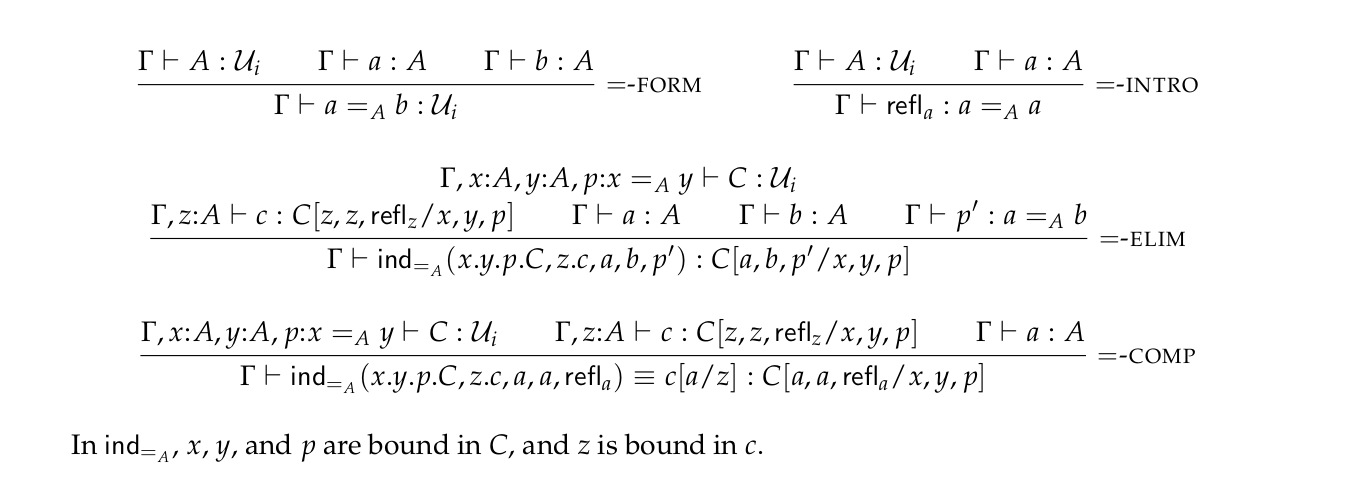
\includegraphics[scale=0.25]{IdentityTypesSmall.png}
}}

Powyższe reguły opisują rodzinę typów, która zazwyczaj nazywana bywa typem identycznościowym (ang. identity type), ale zgodnie z interpretacją homotopiczną będę go nazywał typem ścieżek.

\end{frame}

\begin{frame}{Ścieżki 2 - interpretacja reguł}
\begin{itemize}
	\item Reguła formacji: jeżeli mamy typ $A$ i dwa jego elementy $a, b$, to możemy sformować typ $a =_A b$. Jest to typ, którego elementami są ścieżki z $a$ do $b$. Jeżeli mamy element tego typu, to $a$ i $b$ są równe. Jeżeli typ $A$ jasno wynika z kontekstu, to będziemy pisać po prostu $a = b$ zamiast $a =_A b$.
	\item Reguła wprowadzania: każda rzecz jest równa sama sobie. Ścieżka poświadczająca ten fakt nazywa się $\text{refl}$. Jest to skrót od ang. reflexivity, czyli zwrotność.
	\item Reguła eliminacji: $C$ jest tutaj rodziną typów zależącą od ścieżki $p : x = y$. Reguła głosi, że żeby zdefiniować element $C(x, y, p)$ wystarczy mieć element $C(x, x, \refl{x})$.
	\item Reguła obliczania: chodzi o to, że jeżeli wyeliminujemy element $C(z, z, \refl{z})$, to dostaniemy go spowrotem, tylko po odpowiednim podstawieniu.
\end{itemize}
\end{frame}

\begin{frame}{Ścieżki 3 - indukcja po ścieżkach}
\begin{itemize}
	\item Reguła eliminacji dla ścieżek nosi nazwę indukcji po ścieżkach (ang. path induction).
	\item Zaprezentowany powyżej wariant precyzyjniej nazywa się unbased path induction. Polega na zastąpieniu dwóch obiektów $a, b$ i ścieżki $p$ przez generyczny obiekt $z$ i ścieżkę $\refl{z}$.
	\item Inny wariant nosi nazwę based path induction. Polega on na zastąpieniu obiektu $b$ przez obiekt $a$ oraz ścieżki $p : a = b$ przez ścieżkę $\refl{a}$.
	\item Oba warianty są równoważne. Dowód: HoTT Book, podrozdział 1.12.2.
\end{itemize}
\end{frame}

\begin{frame}{Ścieżki 4 - interpretacja indukcji po ścieżkach}
\begin{itemize}
	\item Tak jak indukcję na liczbach naturalnych możemy zobrazować za pomocą domina, tak indukcję po ścieżkach możemy wyobrażać sobie jako ściągnięcie/zwinięcie ścieżki $p : a = b$ do ścieżki trywialnej.
	\item W wariancie unbased oba końce ścieżki $p$ są wolne. Wybieramy jakiś punkt $z$ na ścieżce i ciągniemy oba końce w jego kierunku. Ostatecznie dostajemy ścieżkę $\refl{z}$.
	\item W wariancie based lewy koniec ścieżki $p$ jest sztywny, a prawy jest wolny. Chwytamy więc prawy koniec $b$ i ciągniemy go po ścieżce w kierunku lewego końca $a$. Ostatecznie dostajemy ścieżkę $\refl{a}$.
	\item Zauważmy, że jeżeli oba końce ścieżki są sztywne, to nie możemy robić indukcji - spróbuj pociągnąć linę okręconą wokół latarni. O tym, czy koniec jest sztywny czy wolny, decyduje to, czy jest skwantyfikowany uniwersalnie czy nie.
\end{itemize}
\end{frame}

\begin{frame}{Ścieżki 5 - wątpliwości i ciekawostki}
\begin{itemize}
	\item Reguła eliminacji dla typu $\text{bool}$ intuicyjnie mówi, że jedynymi elementami typu $\text{bool}$ są $\text{true}$ oraz $\text{false}$.
	\item Czy więc indukcja po ścieżkach mówi, że jedyną ścieżką jest $\text{refl}$?
	\item Zanim odpowiemy, garść ciekawostek.
	\item Indukcja po ścieżkach nie jest HoTTową innowacją. Jedynie nazwa jest nowa. W teorii typów bywa często nazywana $J$.
	\item Zdanie mówiące, że każda ścieżka jest trywialna, nazywa się ``Aksjomat $K$''.
	\item Związek z facetami w czerni jest przypadkowy.
	\item Inne zdanie, mówiące że jest tylko jedna ścieżka, nazywa się w ang. UIP, co jest skrótem od ``Uniqueness of Identity Proofs''.
	\item To właśnie badanie nad tego typu zagadnieniami doprowadziły do homotopicznej interpretacji teorii typów.
\end{itemize}
\end{frame}

\begin{frame}{Ścieżki 6 - rozwianie wątpliwości}
\begin{itemize}
	\item Indukcja po ścieżkach nie głosi, że jest tylko jedna ścieżka.
	\item Formalna różnica jest taka, że typ $\text{bool}$ jest generowany induktywnie, podczas gdy w przypadku ścieżek, które są rodziną typów, to cała rodzina jest generowana induktywnie, a nie pojedynczy typ $x = y$.
	\item Parafrazując, nie można w tym przypadku rozważać samych ścieżek w oderwaniu od ich końców.
	\item Nie możemy zatem udowodnić, że każda ścieżka $p : x = x$ jest trywialna.
	\item Ale możemy udowodnić, że każda ścieżka razem z jej końcami jest trywialna: zachodzi $(x, y, p) = (x, x, \refl{x})$, gdzie równość jest w typie $\Sigma x\ y : A, x = y$. Odpowiada to indukcji po ścieżkach w wersji unbased.
	\item Podobnie dla ustalonego $a : A$ możemy pokazać, że $(x, p) = (a, \refl{a})$ w typie $\Sigma x : A, a = x$. Odpowiada to indukcji po ścieżkach w wersji based.
\end{itemize}
\end{frame}

\begin{frame}{Ścieżki 7 - skąd się biorą ścieżki}
\begin{itemize}
	\item Póki co wiemy, że jest ścieżka trywialna.
	\item Wiemy też, że indukcja po ścieżkach nie wyklucza istnienia innych ścieżek.
	\item Rodzi się jednak pytanie: skąd się biorą ścieżki?
	\item Cztery główne źródła ścieżek, które zobaczymy w przyszłości, to:
	\begin{itemize}
		\item Aksjomat ekstensjonalności dla funkcji - ścieżki powstają z homotopii.
		\item Aksjomat uniwalencji - ścieżki powstają z równoważności.
		\item Wyższe typy induktywne - możemy wrzucić do typu dowolne ścieżki.
		\item Struktura $\omega$-grupoidu - powyższe trzy rodzaje (potencjalnie) nietrywialnych ścieżek mogą ze sobą oddziaływać za pośrednictwem struktury $\omega$-grupoidu, tworząc jeszcze więcej nietrywialnych ścieżek. 
	\end{itemize}
\end{itemize}
\end{frame}

\begin{frame}{Operacje na ścieżkach 1 - definicje}

Uwaga: w nagłówkach definicji i lematów pojawiają się numery, które pokazują, gdzie w HoTTBooku można znaleźć daną definicję/twierdzenie. Link do samego HoTTBooka będzie na końcu slajdów.

\begin{block}{2.1.1 Ścieżka odwrotna}
$\inv{(-)} : \Pi A : \U. \Pi x\ y : A. x = y \to y = x$ \\
$\inv{\refl{x}} \defn \refl{x}$
\end{block}

\begin{block}{2.1.2 Sklejanie ścieżek}
$\sq : \Pi A : \U. \Pi x\ y\ z : A. x = y \to y = z \to x = z$ \\
$\refl{x} \sq \refl{x} \defn \refl{x}$
\end{block}

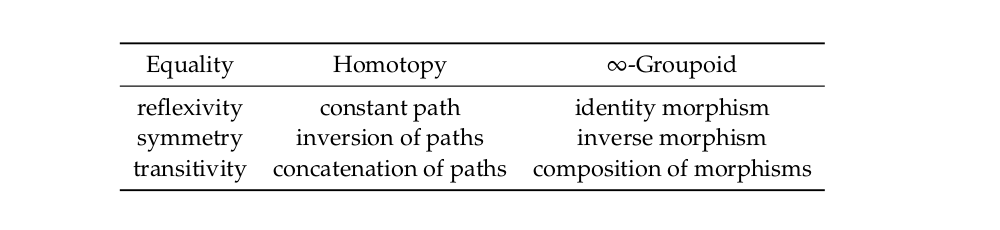
\includegraphics[scale=0.3]{EqPathGrupoid.png}

\end{frame}

\begin{frame}{Operacje na ścieżkach 2 - właściwości}

\begin{block}{2.1.4 Właściwości operacji na ścieżkach}

Niech $A : \U$ będzie typem, $x, y, z, w : A$ punktami, zaś $p : x = y, q : y = z, r : z = w$ ścieżkami. Wtedy:

\begin{itemize}
	\item $\refl{x} \sq p = p$
	\item $p \sq \refl{y} = p$
	\item $p \sq \inv{p} = \refl{x}$
	\item $\inv{p} \sq p = \refl{y}$
	\item $p \sq (q \sq r) = (p \sq q) \sq r$
\end{itemize}

\end{block}

Ćwiczenie: udowodnij.

\end{frame}

\begin{frame}{Prostujcie ścieżki Pana}
\begin{itemize}
	\item Zauważmy, że cała wyższogrupoidowa struktura typów wynika wprost z indukcji po ścieżkach.
	\item Zauważmy też, że powyższe właściwości operacji na ścieżkach są wyrażone za pomocą ścieżek między ścieżkami.
	\item Tak naprawdę, to te właściwości są operacjami, które biorą na wejściu ścieżki i zwracają ścieżki między ścieżkami.
	\item Wobec tego można domniemywać, że te właściwości same spełniają jakieś właściwości, które są wyrażane przez ścieżki jeszcze wyższego rzędu...
	\item ... i tak do nieskończoności.
	\item Katolicy bywają zachęcani do tego, żeby ``prostować ścieżki Pana''. Atoli zachęcam ja was: prostujcie $\omega$-grupoid Pana (oczywiście za pomocą indukcji po ścieżkach).
\end{itemize}
\end{frame}

\begin{frame}{Aplikacja funkcji do ścieżki 1 - definicja}

\begin{block}{2.2.1 Aplikacja funkcji do ścieżki}

$\text{ap} : \Pi A\ B : \U. \Pi f : A \to B. x =_A y \to f(x) =_B f(y)$ \\
$\ap{f}{\refl{x}} \defn \refl{f(x)}$

\end{block}

Klasycznie powyższą definicję moglibyśmy odczytać jako twierdzenie mówiące, że wszystkie funkcje zachowują równość. \\~\

W interpretacji homotopicznej twierdzenie to (które jednocześnie definiuje pewną funkcję) głosi, że funkcje zachowują ścieżki. \\~\

Zauważ też, że również tutaj nie wyczerpujemy tematu. Funkcje zachowują nie tylko ścieżki jednowymiarowe, ale także np. pięciowymiarowe pętle. Podobnie zachowują się funkcje zależne, o których tutaj milczymy.

\end{frame}

\begin{frame}{Aplikacja funkcji do ścieżki 2 - właściwości}
\makebox[\linewidth]{\parbox{12cm}
{
	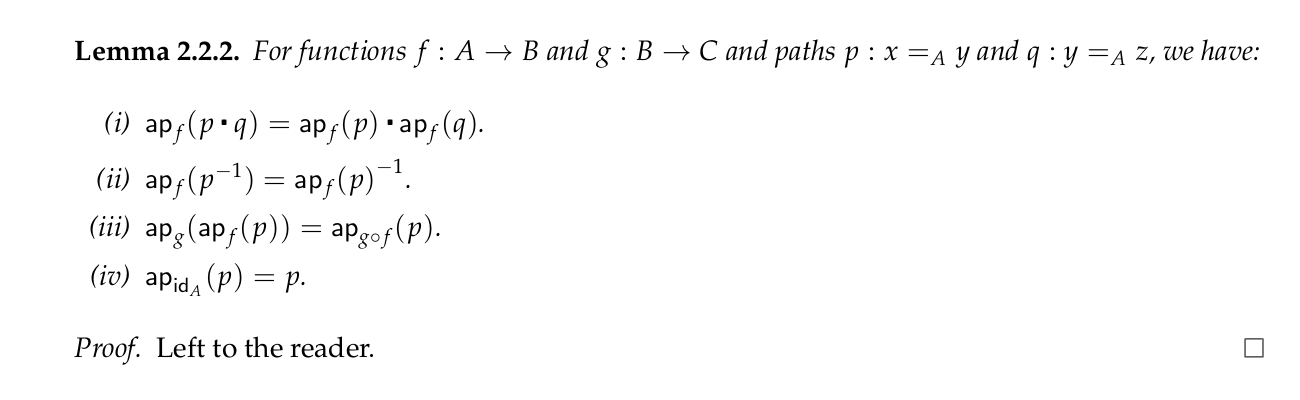
\includegraphics[scale=0.25]{ap.png}
}}

Ćwiczenie: udowodnij.

\end{frame}

\begin{frame}{Transport 1 - definicja}

\begin{block}{2.3.1 Transport}

$\text{transport} : \Pi A : \U. \Pi P : A \to \U. \Pi x\ y : A. x = y \to P(x) \to P(y)$ \\
$\text{transport}(\refl{x}) \defn \text{id}_{P(x)}$ \\~\

Notacja: $p_* \defn \text{transport}(p)$

\end{block}

Powyższe klasycznie można odczytać jako jedną stronę równoważności, której Leibniz użył do zdefiniowania równości: ``dwie rzeczy są równe wtedy i tylko wtedy, gdy mają takie same właściwości''.\\~\

Homotopicznie sprawa jest nieco ciekawsza: jeżeli mamy ścieżkę $p : x =_A y$ i jakiś obiekt typu $P(x)$, to możemy go przenieść (czyli właśnie przetransportować) do typu $P(y)$ wzdłuż ścieżki $p$.

\end{frame}

\begin{frame}{Transport 2 - właściwości}

\makebox[\linewidth]{\parbox{12cm}
{
	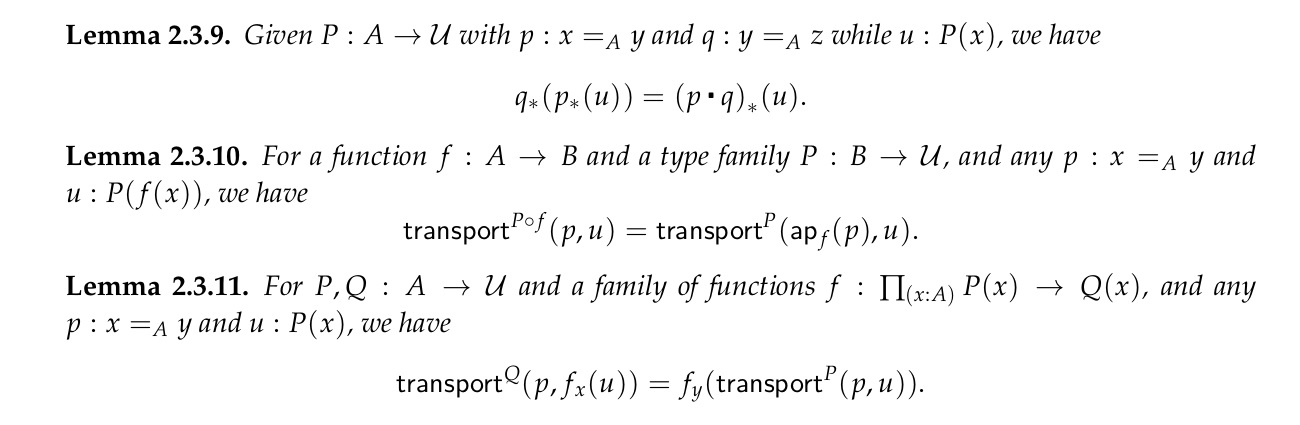
\includegraphics[scale=0.25]{transport.png}
}}

Ćwiczenie: udowodnij.

\end{frame}

\begin{frame}{Aplikacja funkcji zależnej do ścieżki}

\begin{block}{Lemat 2.3.4 Aplikacja funkcji zależnej do ścieżki}

$\text{apd} : \Pi A : \U. \Pi P : A \to \U. \Pi f : (\Pi x : A. P(x)). \Pi p : x = y. p_*(f(x)) = f(y)$ \\
$\apd{f}{\refl{x}} \defn \refl{f(x)}$

\end{block}

Aplikacja funkcji zależnych do ścieżek jest analogiczna do aplikacji funkcji niezależnych do ścieżek, ale jest mały twist - musimy użyć transportu, bo wyniki funkcji dla $x$ i $y$ żyją w różnych typach.

\end{frame}

\begin{frame}{Homotopie 1 - definicje i właściwości}

\makebox[\linewidth]{\parbox{12cm}
{
	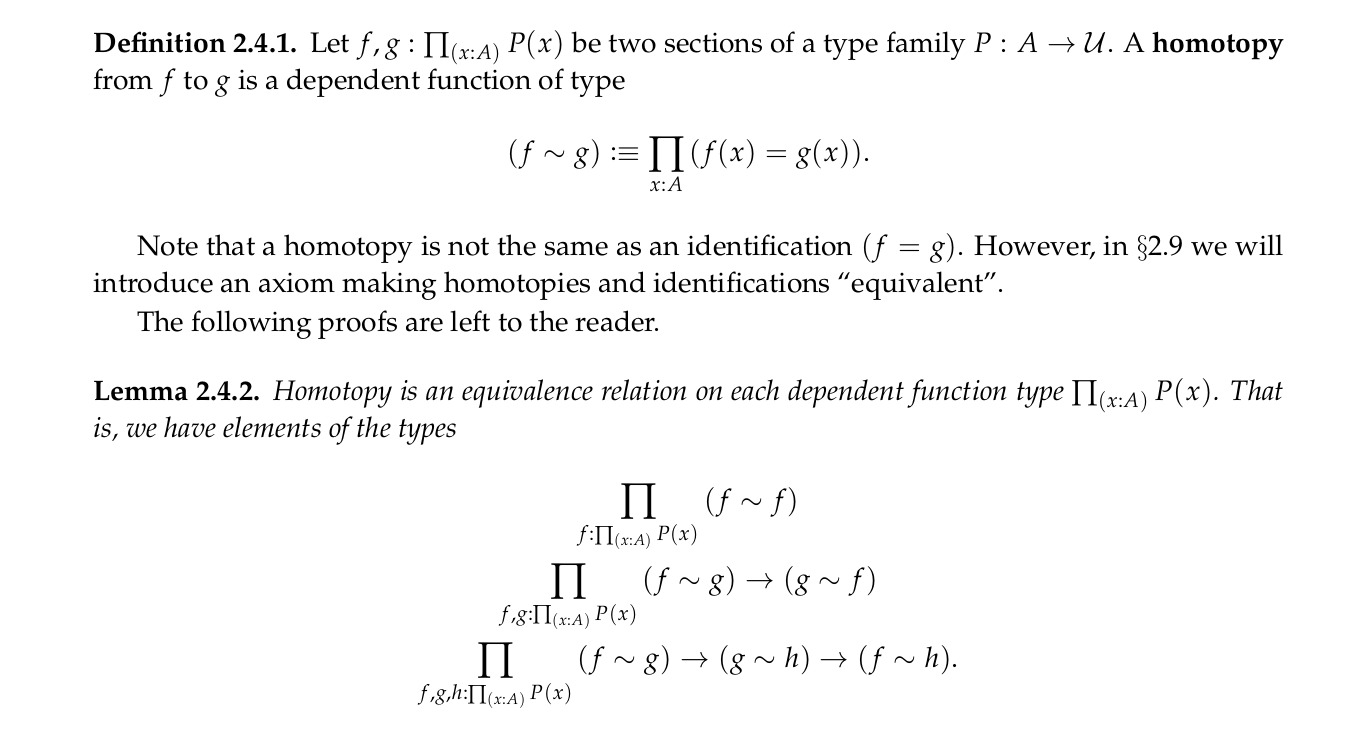
\includegraphics[scale=0.25]{homotopy.png}
}}

Ćwiczenie: udowodnij.

\end{frame}

\begin{frame}{Homotopie 2 - intuicja}
\begin{itemize}
	\item Klasycznie (czyli płasko) $f \sim g$ możemy czytać jako ``$f$ i $g$ są ekstensjonalnie równe''.
	\item HoTTowym odpowiednikiem ekstensjonalnej równości jest homotopia, która intuicyjnie znaczy, że dla każdego elementu dziedziny wyniki funkcji $f$ i $g$ są połączone ścieżką w przeciwdziedzinie.
	\item To pojęcie homotopii różni się jednak od tego zaprezentowanego w pierwszych slajdach, gdyż homotopie i ścieżki między funkcjami nie są a priori tym samym - nie da się tego pokazać w podstawowej wersji naszej teorii.
	\item Dlatego w bliskiej przyszłości będziemy dążyć do tego, żeby załatać tę sytuację za pomocą aksjomatu ekstensjonalności.
\end{itemize}
\end{frame}

\section{Równoważności}

\subsection{Część 1}

\begin{frame}{Równoważności 1 - pomysły}

Homotopicznie zinterpretowawszy typy, zdążajmy teraz ku aksjomatowi uniwalencji. Żeby go sformułować, potrzebne nam będzie pojęcie równoważności typów. Przyjrzyjmy się zatem tradycyjnym pojęciom o podobnym charakterze:

\begin{itemize}
	\item Bijekcja - funkcja będąca surjekcją i injekcją.
	\item Bijekcja v2 - dla każdego elementu przeciwdziedziny istnieje dokładnie jeden element dziedziny.
	\item Izomorfizm - morfizm mający obustronną odwrotność.
\end{itemize}
\end{frame}

\begin{frame}{Równoważności 2 - kwaziodwrotność}

\begin{block}{Kwaziodwrotność}
$\qinv : \Pi A\ B : \U. (A \to B) \to \U$ \\
$\displaystyle \qinv(f) \defn \sum_{g : B \to A} g \comp f \sim \id_A \times f \comp g \sim \id_B$
\end{block}

Funkcję mającą odwrotność (wraz z dowodami na to, że faktycznie jest to odwrotność) będziemy nazywać kwaziodwrotnością. \\~\

Ćwiczenio-przykład. Pokaż, że kwaziodwrotnościami są następujące funkcje:
\begin{itemize}
	\item $\id_A : A \to A$
	\item $(p \sq -) : y = z \to x = z$
	\item $(- \sq q) : x = y \to x = z$
	\item $\transport(p, -) : P(x) \to P(y)$
\end{itemize}

\end{frame}

\begin{frame}{Równoważności 3 - co poszło nie tak}

Dlaczego nazwaliśmy funkcje mające odwrotność kwaziodwrotnościami, a nie izomorfizmami? Okazuje się, że są one wadliwe. Jeżeli narysujemy odpowiednio plastyczny rysunek, to ujrzymy uzasadnienie dla poniższego twierdzenia:

\begin{block}{Twierdzenie 4.1.1 Kwaziodwrotności to pętle}

$\Pi A\ B : \U. \Pi f : A \to B. \qinv(f) \to (\qinv(f) = \Pi x : A. x = x)$

\end{block}

Twierdzenie to głosi, że jeżeli funkcja $f$ jest kwaziodwrotnością, to typ $\qinv(f)$ jest równy typowi funkcji zależnych, które każdemu punktowi przyporządkowują jakąś pętlę. Dlaczego twierdzenie to nas niepokoi? Jak już wiemy, pętli w danym punkcie może być wiele. Mimo, że dana funkcja może mieć tylko jedną odwrotność, to dowodów tego faktu (czyli odpowiednich par ścieżek) może być wiele. Wobec tego funkcja może być kwaziodwrotnością na wiele sposobów.

\end{frame}

\begin{frame}{Równoważności 4 - pobożne życzenia}
\begin{itemize}
	\item Chcielibyśmy, żeby definicja równoważności $\isequiv$ spełniała następujące warunki:
	\begin{itemize}
		\item $\qinv(f) \to \isequiv(f)$
		\item $\isequiv(f) \to \qinv(f)$
		\item $\Pi e_1\ e_2 : \isequiv(f). e_1 = e_2$
	\end{itemize}
	\item Parafrazując: $\isequiv$ to niemal to samo co $\qinv$, ale każda funkcja może być równoważnością na co najwyżej jeden sposób.
\end{itemize}
\end{frame}

\begin{frame}{Równoważności 5 - definicje}

Niech $A, B : \U$ będą typami, a $f : A \to B$ funkcją.

\begin{block}{Równoważność 1}
$
\displaystyle
	\isequiv_1(f) \defn
		\left(\sum_{g : B \to A} f \comp g \sim \id_B\right) \times
		\left(\sum_{h : B \to A} h \comp f \sim \id_A\right)
$
\end{block}

\begin{block}{Równoważność 2}
$
\displaystyle
	\isequiv_2(f) \defn
		\sum_{g : B \to A} \sum_{\eta : g \comp f \sim \id_A} \sum_{\epsilon : f \comp g \sim \id_B}
			\prod_{x : A} \ap{f}{\eta(x)} = \epsilon(\ap{f}{x})
$
\end{block}

\end{frame}


\begin{frame}{Równoważności 6 - wybór}

Żeby uzyskać definicję $\isequiv$, możemy ``ulepszyć'' definicję $\qinv$. Możemy to zrobić na dwa sposoby:

\begin{itemize}
	\item Rozdzielamy odwrotność na dwie osobne. Wtedy każda z nich ma swój osobny dowód, że jest odwrotnością i gitara gra.
	\item Dodajemy dodatkową ścieżkę, która zapewnia, że ścieżki dowodzące odwrotności dobrze się ze sobą zachowują.
\end{itemize}

Druga definicja zdaje się być korzystniejsza w użyciu, bo łatwiej wyjąć z niej odwrotność. Dużo łatwiej jest też dostrzec, że spełnia ona dwa pierwsze pożądane przez nas warunki. Tego, że spełnia trzeci, nie będziemy dowodzić, bo to nudne.

\end{frame}

\begin{frame}{Równoważności 7 - więcej definicji}

\begin{block}{Równoważność 3}
$
\displaystyle
	\isequiv_3(f) \defn
		\prod_{y : B} \text{isContr}\left(\sum_{x : A} f(x) = y\right)
$
\end{block}


\begin{block}{Równoważność 4}
$
\displaystyle
	\isequiv_4(f) \defn ||\qinv(f)||
$
\end{block}

Możliwe są jeszcze dwie inne definicje równoważności, których jednak nie wybierzemy, gdyż zawierają nieznane nam pojęcia.

\end{frame}

\begin{frame}{Równoważności 8 - interpretacja reszty definciji}
\begin{itemize}
	\item Definicja nr 4 to coś w stylu: $\qinv$ nie działa, więc ulepszymy go czarami tak, żeby jednak działał (więcej dowiemy się później).
	\item Definicja nr 3 odpowiada naszej definicji bijekcji v2 (dla każdego elementu przeciwdziedziny istnieje dokładnie jeden element dziedziny), ale musimy zapisać to bardziej homotopicznie.
	\item Jest tak dlatego, że interesują nas nie tylko punkty, ale też ścieżki na każdym możliwym poziomie.
	\item Definicję tę można czytać tak: dla każdego punktu przeciwdziedziny istnieje tylko jeden punkt dziedziny i jedna pętla na nim, i jedna pętla na tej pętli, i jedna pętli na tej pętli i tak dalej na każdym poziomie.
	\item Prościej: przeciwobraz każdego punktu przeciwdziedziny jest równoważny typowi $\textbf{1}$.
\end{itemize}
\end{frame}

\begin{frame}{Równoważności 9 - refleksja}
\begin{itemize}
	\item Oczywiście wszystkie 4 definicje są równoważne.
	\item Dla precyzji jednak przyjmujemy $\isequiv(f) \defn \isequiv_1(f)$, tzn. domyślnie będziemy posługiwać się definicją z dwiema osobnymi odwrotnościami.
	\item Skąd jednak biorą się problemy? Klasyczna definicja izomorfizmu okazała się za słaba, zaś definicję bijekcji v2 również trzeba było odpowiednio stuningować.
	\item Powód tego jest prosty: klasyczne definicje pochodzą ze świata teorii zbiorów, w którym to świecie mamy tylko worki z kropkami. W świecie, w którym kropki mogą być połączone, definicje trzeba unowocześnić.
	\item Żeby lepiej zrozumieć różnicę, dokonajmy pewnego wielkiego odkrycia.
\end{itemize}
\end{frame}

\subsection{Część 2}

\begin{frame}{Wielkie odkrycie 1 - injekcja to surjekcja}
\begin{itemize}
	\item W ramach ciekawostki dokonajmy pewnego wesołego odkrycia: injekcja to surjekcja.
	\item Klasycznie $f$ jest surjekcją, gdy $\forall y \in B. \exists x \in A. f(x) = y$
	\item Klasycznie $f$ jest injekcją, gdy $\forall x\ y \in A. f(x) = f(y) \implies x = y$
	\item Przeformułujmy tę definicję na taką bardziej homo, wciskając tam więcej ścieżek: $f$ jest injekcją, gdy $\Pi x\ y : A. \Pi q : f(x) = f(y). \Sigma p : x = y. \ap{f}{p} = q$
	\item Klasyczną surjekcję możemy rozumieć jako 0-surjekcję, tzn. surjekcję na punktach, zaś klasyczną injekcję jako 1-surjekcję, tzn. surjekcję na ścieżkach między punktami.
	\item Jak więc widać, klasyczna bijekcja to surjekcja na poziomach $0$ i $1$. A co z wyższymi?
	\item Próba pogłębienia tej obserwacji prowadzi do ciekawego twierdzenia.
\end{itemize}
\end{frame}

\begin{frame}{Wielkie odkrycie 2 - wesoła charakteryzacja równoważności}

Niech $A, B : \U$ będą typami, a $f: A \to B$ funkcją.

\begin{block}{Surjekcja - nieco inaczej niż w książce}
$f$ jest surjekcją, gdy $\Pi y : B. \Sigma x : A. f(x) = y$
\end{block}

\begin{block}{Zanurzenie}
$f$ jest zanurzeniem, gdy dla każdego $x, y : A$ funkcja $\text{ap}_f : x = y \to f(x) = f(y)$ jest równoważnością.
\end{block}

\begin{block}{Wesoła charakteryzacja równoważności}
$f$ jest równoważnością wtedy i tylko wtedy, gdy jest surjekcją i zanurzeniem.
\end{block}

\end{frame}

\begin{frame}{Wielkie odkrycie 3 - wnioski}
\begin{itemize}
	\item Nasze twierdzenie możemy odwinąć: $f$ jest równoważnością gdy jest surjekcją i $\text{ap}_f$ jest surjekcją i $\text{ap}_{\text{ap}_f}$ jest surjekcją etc.
	\item Wobec tego $f$ jest równoważnością, gdy jest surjekcją na wszystkich poziomach - na punktach, ścieżkach między punktami, ścieżkach między ścieżkami etc.
	\item Stąd wnioskujemy, że klasyczne definicje okazują się za słabe, gdyż dotyczą tylko punktów (surjekcja) i ścieżek (injekcja), a zatem poziomów $0$ i $1$, a my mamy do czynienia z potencjalnie nieskończenie wieloma poziomami.
\end{itemize}
\end{frame}

\begin{frame}{Filozoficzna interpretacja równoważności}
\begin{itemize}
	\item Przypomnijmy, że z dowolnej definicji równoważności jesteśmy w stanie uzyskać następujące rzeczy: funkcje $f : A \to B$ i $\inv{f} : B \to A$ oraz homotopie $\eta : \inv{f} \comp f \sim \id_A$ i $\epsilon : f \comp \inv{f} \sim \id_B$
	\item Okazuje się, że równoważność $A \simeq B$ możemy zinterpretować jako zestaw czterech reguł opisujących typ $B$ w terminach typu $A$.
	\item Funkcja $f : A \to B$ to reguła wprowadzania.
	\item Funkcja $\finv{f} : B \to A$ to reguła eliminacji.
	\item Homotopia $\eta$ to zdaniowa reguła obliczania.
	\item Homotopia $\epsilon$ to zdaniowa reguła unikalności.
	\item Powyższe rozważania okażą się przydatne za chwilę, gdy będziemy chcieli scharakteryzować przestrzenie ścieżek dla różnych typów.
\end{itemize}
\end{frame}

\section{Charakteryzacje ścieżek}

\subsection{Część 1}

\begin{frame}{Charakteryzacje ścieżek 1 - wprowadzenie}
\begin{itemize}
	\item W klasycznej matematyce mamy twierdzenia mówiące, kiedy jakieś obiekty są równe, np. $(a, b) = (a', b') \iff a = a' \land b = b'$.
	\item W HoTT mamy podobnie wyglądające twierdzenia: $(a, b) = (a', b') \simeq a = a' \times b = b'$.
	\item Zgodnie jednak z interpretacją homotopiczną są one dużo ogólniejsze od swoich klasycznych przodków, gdyż charakteryzują one przestrzenie ścieżek w danym typie.
\end{itemize}
\end{frame}

\begin{frame}{Charakteryzacje ścieżek 2 - plan}
\begin{itemize}
	\item Jakkolwiek sprawa brzmi prosto, zróżnicowanie w tej materii jest spore.
	\item Za chwilę zobaczymy charakteryzację ścieżek w typach banalnych oraz w typach negatywnych (czyli takich, w których kluczowa jest reguła eliminacji).
	\item Później zobaczymy, że niektórych pożądanych charakteryzacji nie da się udowodnić i załatamy je aksjomatami.
	\item Następnie zobaczymy sposób pozwalający charakteryzować ścieżki w typach pozytywnych (czyli takich, w których kluczowe są reguły wprowadzania).
	\item HoTT pozwala nam jednak zdefiniować typy, dla których charakteryzacja ścieżek jest (częściowo) otwartym problemem badawczym, np. $n$-wymiarowe kule, torusy, podwieszenia i inne skomplikowane przestrzenie.
\end{itemize}
\end{frame}

\begin{frame}{Charakteryzacje ścieżek 3 - typy banalne i negatywne}

\begin{block}{Ścieżki między elementami typu pustego}
$\Pi x\ y : \textbf{0}. (x = y) \simeq \textbf{1}$
\end{block}

\begin{block}{2.8 Ścieżki między elementami typu unit}
$\Pi x\ y : \textbf{1}. (x = y) \simeq \textbf{1}$
\end{block}

\begin{block}{2.5.1 Ścieżki między parami}
$\Pi A\ B : \U. \Pi a\ a' : A. \Pi b\ b': B. ((a, b) = (a', b')) \simeq a = a' \times b = b'$
\end{block}

\begin{block}{2.7.2 Ścieżki między parami zależnymi}
$\Pi A : \U. \Pi B : A \to \U. \Pi w\ w' : \sum_{x : A} B(x).$ \\
$\displaystyle \quad (w = w') \simeq \sum_{p : \prl(w) = \prl(w')} p_*(\prr(w)) = \prr(w')$
\end{block}

\end{frame}

\begin{frame}{Charakteryzacje ścieżek 4 - interpretacja}
\begin{itemize}
	\item Między każdymi dwoma elementami typu pustego jest dokładnie jedna ścieżka. Albo i nie, albo i dwie. Nie ma to większego znaczenia, bo jeżeli wpadnie nam w ręce element typu pustego, to i tak mamy sprzeczność.
	\item Między elementami $\textbf{1}$ jest dokładnie jedna ścieżka.
	\item Ścieżki między parami to pary ścieżek.
	\item Ścieżki między parami zależnymi to zależne pary ścieżek.
\end{itemize}
\end{frame}

\begin{frame}{Ekstensjonalność 1 - aksjomat ekstensjonalności}

Jeżeli dwie funkcje są równe, to są też homotopiczne (czyli ekstensjonalnie równe).

\begin{block}{2.9.2 Aplikacja homotopii do argumentu}
$\happly: \Pi A\ B : \U. \Pi f\ g : A \to B. f = g \to \Pi x : A. f(x) = g(x)$ \\
$\happly(\refl{f}) = \lambda x : A. \refl{f(x)}$
\end{block}

Jednak implikacji w drugą stronę (ani tym bardziej równoważności) nie da się pokazać. Wobec tego wprowadzamy aksjomat:

\begin{block}{2.9.3 Aksjomat ekstensjonalności dla funkcji}
Funkcja $\happly$ jest równoważnością.
\end{block}

\begin{block}{Wniosek: charakteryzacja ścieżek między funkcjami}
$(f = g) \simeq \Pi x : A. f(x) = g(x)$
\end{block}

\end{frame}

\begin{frame}{Ekstensjonalność 2 - rozbicie na reguły}

Zauważmy, że charakteryzacje ścieżek możemy rozbić na reguły przypominające reguły opisujące typy, w których te ścieżki żyją. Jest to prawdą nie tylko dla aksjomatu ekstensjonalności, ale też np. dla twierdzeń charakteryzujących ścieżki między parami.

\begin{block}{Reguły opisujące ścieżki między funkcjami}
$\funext : \Pi A\ B : \U. \Pi f\ g : A \to B. (\Pi x : A. f(x) = g(x)) \to f = g$ \\

$\happly(\funext(h), x) = h(x)$ \\

$\funext(\lambda x : A. \happly(p, x)) = p$
\end{block}

\end{frame}

\begin{frame}{Ekstensjonalność 3 - interpretacja}
\begin{itemize}
	\item Reguła formacji dla $f = g$ pochodzi bezpośrednio z induktywnej definicji ścieżek.
	\item Reguła wprowadzania to $\funext$: żeby zrobić ścieżkę $f = g$, wystarczy nam homotopia.
	\item Reguła eliminacji to $\happly$: jeżeli mamy ścieżkę $f = g$, to możemy uzyskać ścieżkę $f(x) = g(x)$ dla dowolnego $x$ należącego do dziedziny.
	\item Reguła obliczania mówi, że jeżeli zaaplikujemy do $x : A$ ścieżkę zrobioną z homotopii $h : \Pi x : A. f(x) = g(x)$ za pomocą $\funext$, to dostaniemy $h(x)$.
	\item Reguła unikalności mówi, że każda ścieżka między funkcjami pochodzi od ekstensjonalności zaaplikowanej do odpowiedniej homotopii.
\end{itemize}
\end{frame}

\begin{frame}{Ekstensjonalność 4 - charakteryzacja operacji}

Możemy scharakteryzować nie tylko ścieżki między funkcjami, ale także operacje na tych ścieżkach.

\begin{block}{Charakteryzacja operacji na ścieżkach między funkcjami}
$\refl{f} = \funext(\lambda x : A. \refl{f(x)})$ \\

$\inv{p} = \funext(\lambda x : A.\inv{\happly(p, x)})$ \\

$p \sq q = \funext(\lambda x : A. \happly(p, x) \sq \happly(q, x))$
\end{block}

Intuicja jest prosta:
\begin{itemize}
	\item Funkcja bierze argument i zwraca wynik.
	\item Ścieżka między funkcjami to funkcja biorąca argument i zwracająca ścieżkę między wynikami.
	\item Operacja na ścieżkach między funkcjami pochodzi na mocy ekstensjonalności od funkcji biorącej argument i wykonującej operację na ścieżkach między wynikami.
\end{itemize}

\end{frame}

\begin{frame}{Ekstensjonalność 5 - charakteryzacja transportu}

Możemy też scharakteryzować transport w rodzinach typów postaci $\lambda x : X. A(x) \to B(x)$. \\~\

Dla typu $X : \U$, rodzin typów $A, B : X \to \U$, elementów $x_1, x_2 : X$, funkcji $f : A(x_1) \to B(x_1)$ oraz ścieżki $p : x_1 = x_2$ mamy:

\begin{block}{Charakteryzacja transportu dla funkcji}
$\transport^{\lambda x : X. A(x) \to B(x)}(p, f) =$ \\
$\quad \lambda a : A(x_2). \transport^B(p, f(\transport^A(\inv{p}, a)))$
\end{block}

Interpretacja twierdzenia jest łatwa: chcemy zrobić funkcję typu $A(x_2) \to B(x_2)$. Bierzemy więc element $a : A(x_2)$, transportujemy go ścieżką $p$ w tył do typu $A(x_1)$, używamy funkcji $f$ by dostać element typu $B(x_1)$ i transportujemy go wzdłuż $p$ do typu $B(x_2)$.

\end{frame}

\begin{frame}{Uniwalencja 1 - aksjomat uniwalencji}

Jeżeli dwa typy są równe, to są też równoważne.

\begin{block}{2.10.2 Jak przerobić ścieżkę na równoważność}
$\idtoeqv: \Pi A\ B. A = B \to A \simeq B$ \\
$\idtoeqv(p) = \transport^{\id_\U}(p)$ \\

Słownie: $\idtoeqv$ to specjalny przypadek transportu. Trzeba jeszcze przez indukcję po ścieżkach pokazać, że jest to równoważność.
\end{block}

Podobnie jak w przypadku ekstensjonalności dla funkcji, w drugą stronę implikacji pokazać się nie da i stąd aksjomat.

\begin{block}{2.10.3 Aksjomat uniwalencji}
Funkcja $\idtoeqv$ jest równoważnością.
\end{block}

\begin{block}{Aksjomat uniwalencji, tylko ładniej zapisany}
$(A = B) \simeq (A \simeq B)$ lub równoważnie $(A = B) = (A \simeq B)$
\end{block}

\end{frame}

\begin{frame}{Uniwalencja 2 - reguły i charakteryzacje}

\begin{block}{Reguły opisujące ścieżki między typami}
$\ua : \Pi A\ B : \U. (A \simeq B) \to A = B$ \\

$\idtoeqv(\ua(e)) = e$ \\

$\ua(\idtoeqv(p)) = p$
\end{block}

\begin{block}{Charakteryzacja operacji na ścieżkach między typami}
$\refl{f} = \ua(\id_A)$ \\

$\inv{p} = \ua(\inv{\idtoeqv(p)})$ \\

$p \sq q = \ua(\idtoeqv(q) \comp \idtoeqv(p))$
\end{block}

Dla rodziny typów $B : A \to \U$, punktów $x, y : A$, ścieżki $p : x = y$ i elementu $u : B(x)$ mamy:

\begin{block}{Charakteryzacja transportu dla typów}
$\transport^{\lambda X : \U.X}(p, f) = \idtoeqv(\ap{B}{p})(u)$
\end{block}

\end{frame}

\begin{frame}{Uniwalencja 3 - przykład filozoficzny}
\begin{itemize}
	\item Rozważmy dwa poniższe typy (tak naprawdę powinniśmy też podać reguły eliminacji i obliczania, ale nie są one istotne dla przykładu).
	\item Niech $\mathbb{N} \defn 0 \: | \: S\ \mathbb{N}$ i niech $\mathbb{N}' \defn 0' \: | \: S'\ \mathbb{N}'$
	\item Rodzi się pytanie: czy $\mathbb{N}$ i $\mathbb{N}'$ to to samo, czy coś innego?
	\item Odpowiedź klasyczna: istnieje oczywista bijekcja $\mathbb{N} \cong \mathbb{N}'$. Na mocy nadużycia języka będziemy utożsamiać $\mathbb{N}$ i $\mathbb{N}'$, tzn. traktować je tak, jakby $\mathbb{N} = \mathbb{N}'$ mimo, że formalnie tak nie jest.
	\item Odpowiedź HoTTowa: istnieje oczywista równoważność $e : \mathbb{N} \simeq \mathbb{N}'$. Wobec tego na mocy aksjomatu uniwalencji mamy ścieżkę $\text{ua}(e) : \mathbb{N} = \mathbb{N}'$.
\end{itemize}
\end{frame}

\begin{frame}{Uniwalencja 4 - przykład praktyczny}
\begin{itemize}
	\item Aksjomat uniwalencji nie tylko usuwa nieprzyjemny filozoficzny smrodek, ale daje nam też nowe sposoby rozumowania.
	\item Definicja: $f : B \to C$ jest monomorfizmem gdy dla dowolnych $g, h : A \to B$ jeżeli $f \comp g = f \comp h$ to $g = h$.
	\item Twierdzenie: każda równoważność jest monomorfizmem.
	\item Dowód klasyczny: każda równoważność ma odwrotność. Użyj jej.
	\item Dowód HoTTowy: na mocy uniwalencji każda równoważność pochodzi od jakiejś ścieżki. Na mocy indukcji po ścieżkach możemy założyć, że ścieżka ta jest trywialna, a zatem nasza równoważność jest identycznością. Wtedy nasze założenie zamienia się na $\id_B \comp g = \id_B \comp h$ i oblicza się do $g = h$, co mieliśmy pokazać.
\end{itemize}
\end{frame}

\begin{frame}{Filozoficzna interpretacja charakteryzacji i aksjomatów}
\begin{itemize}
	\item Na mocy naszej interpretacji równoważności nasze charakteryzacje opisują przestrzenie ścieżek tak dokładnie, jakby były one osobnymi typami zdefiniowanymi za pomocą reguł.
	\item W przypadkach, w których nie jesteśmy w stanie udowodnić charakteryzacji, dajemy sobie protezę w postaci odpowiednich aksjomatów.
	\item Tak więc aksjomat ekstensjonalności dla funkcji możemy postrzegać jako charakteryzację ścieżek między funkcjami za pomocą reguł.
	\item Podobnie aksjomat uniwalencji możemy postrzegać jako aksjomat ekstensjonalności dla uniwersum, czyli charakteryzację ścieżek między typami za pomocą reguł.
\end{itemize}
\end{frame}

\subsection{Część 2}

\begin{frame}{Metoda encode-decode 1 - wstęp}
\begin{itemize}
	\item Ogólna metoda pozwalająca scharakteryzować ścieżki (niektórych) typów  (głównie pozytywnych) nosi nazwę encode-decode.
	\item Metoda składa się z czterech kroków.
	\item Krok 1: definiujemy rodzinę typów $\code : A \to A \to \U$, której celem jest opisanie typu $x =_A y$ w bardziej ludzki sposób.
	\item Krok 2: deiniujemy funkcję $\encode : \Pi x\ y : A. x = y \to \code(x, y)$
	\item Krok 3: definiujemy funkcję $\decode : \Pi x\ y : A. code(x, y) \to x = y$
	\item Krok 4: pokazujemy, że $\encode$ i $\decode$ są swoimi odwrotnościami.
	\item Dzięki temu dostajemy charakteryzację postaci $\Pi x\ y : A. (x = y) \simeq \code(x, y)$.
\end{itemize}
\end{frame}

\begin{frame}{Metoda encode-decode 1.5 - objaśnienie}
\begin{itemize}
	\item Uwaga: doszły mnie słuchy, że są problemy z odszyfrowaniem poniższego slajdu, więc wyjaśniam.
	\item $\textbf{2}$ (pogrubiona cyfra dwa) oznacza typ dwuelementowy, znany szerzej jako typ \texttt{bool}. Jego dwa elementy to $0_{\textbf{2}}$ oraz $1_{\textbf{2}}$ (chude 0 i 1 z indeksem dolnym $\textbf{2}$). Można je interpretować, odpowiednio, jako \texttt{false} i \texttt{true}, czyli prawdę i fałsz.
	\item $\textbf{0}$ (pogrubiona cyfra zero) oznacza typ pusty, który nie ma żadnych elementów.
	\item $\textbf{1}$ (pogrubiona cyfra jeden) oznacza typ jednoelementowy. Jego jedyny element to $*$, czyli gwiazdka.
\end{itemize}
\end{frame}

\begin{frame}{Metoda encode-decode 2 - definicje dla bool}
	
Scharakteryzujmy ścieżki w typie $\textbf{2}$.

\begin{block}{$\code : \textbf{2} \to \textbf{2} \to \U$}
$\code(0_{\textbf{2}}, 0_{\textbf{2}}) \defn \textbf{1}$ \\
$\code(1_{\textbf{2}}, 1_{\textbf{2}}) \defn \textbf{1}$ \\
$\code(\_, \_) \defn \textbf{0}$
\end{block}

\begin{block}{$\encode : \Pi (x y : \textbf{2}). x = y \to \code(x, y)$}
$\encode_{0_{\textbf{2}}, 0_{\textbf{2}}}(\refl{0_{\textbf{2}}}) \defn *$ \\
$\encode_{1_{\textbf{2}}, 1_{\textbf{2}}}(\refl{1_{\textbf{2}}}) \defn *$
\end{block}

\begin{block}{$\decode : \Pi (x\ y : \textbf{2}). \code(x, y) \to x = y$}
$\decode_{0_{\textbf{2}}, 0_{\textbf{2}}}(*) \defn \refl{0_{\textbf{2}}}$ \\
$\decode_{1_{\textbf{2}}, 1_{\textbf{2}}}(*) \defn \refl{1_{\textbf{2}}}$ \\
$\decode_{0_{\textbf{2}}, 1_{\textbf{2}}}(x) \defn \text{ind}_{\textbf{0}}(\lambda \_. 0_{\textbf{2}} = 1_{\textbf{2}}, x)$ (czyli sprzeczność) \\
$\decode_{1_{\textbf{2}}, 0_{\textbf{2}}}(x) \defn \text{też sprzeczność}$
\end{block}

\end{frame}

\begin{frame}{Metoda encode-decode 3 - twierdzenia dla bool}

\begin{block}{$encode$ jest odwrotnością $decode$}
$\encode(\decode(c)) = c$
\end{block}
	
\begin{block}{$decode$ jest odwrotnością $encode$}
$\decode(\encode(p)) = p$
\end{block}

\begin{block}{Wniosek 1: charakteryzacja ścieżek w typie $\textbf{2}$}
$\Pi x\ y : \textbf{2}. (x = y) \simeq \code(x, y)$
\end{block}

\begin{block}{Wniosek 2: elementy typu $\textbf{2}$ są różne}
$0_{\textbf{2}} \neq 1_{\textbf{2}}$
\end{block}

Ćwiczenie: udowodnij.

\end{frame}

\begin{frame}{Metoda encode-decode 4 - interpretacja dla bool}
\begin{itemize}
	\item Podobnie jak poprzednio, naszą charakteryzację możemy zinterpretować regułowo.
	\item $\decode$ jest tutaj regułą wprowadzania. Dokładnie opisuje ona, jak zrobić każdą z 4 potencjalnie możliwych ścieżek, np. jeżeli chcesz zrobić ścieżkę $0_{\textbf{2}} = 0_{\textbf{2}}$ to daj mi $* : \textbf{1}$, a jeżeli chcesz zrobić ścieżkę $0_{\textbf{2}} = 1_{\textbf{2}}$, to daj mi $x : \textbf{0}$.
	\item $\encode$ to reguła eliminacji. Dla faktycznie równych argumentów nie mówi nam ona nic ciekawego. Dla różnych argumentów daje nam ona natomiast sprzeczność.
	\item Twierdzenie decode-encode to reguła obliczania, a twierdzenie encode-decode to reguła unikalności.
	\item Reguły obliczania i unikalności są mało ciekawe, a dodatkowo mogą się różnić w zależności od sposobu, w jaki udowodniono twierdzenie. W naszym przypadku akurat jest tylko jeden słuszny sposób, ale w przypadku bardziej skomplikowanych typów niekoniecznie.
\end{itemize}
\end{frame}

\begin{frame}{Ścieżki między ścieżkami 1 - twierdzenie i przykłady}

\begin{block}{Twierdzenie}
Jeżeli $f : A \to B$ jest równoważnością, to dla dowolnych $x, y : A$ funkcja $\text{ap}_f : x = y \to f(x) = f(y)$ też jest równoważnością.
\end{block}

\begin{block}{Dowód}
Odwrotnością $\text{ap}_f$ jest oczywiście $\text{ap}_{\finv{f}}$.
\end{block}

\makebox[\linewidth]{\parbox{12cm}
{
	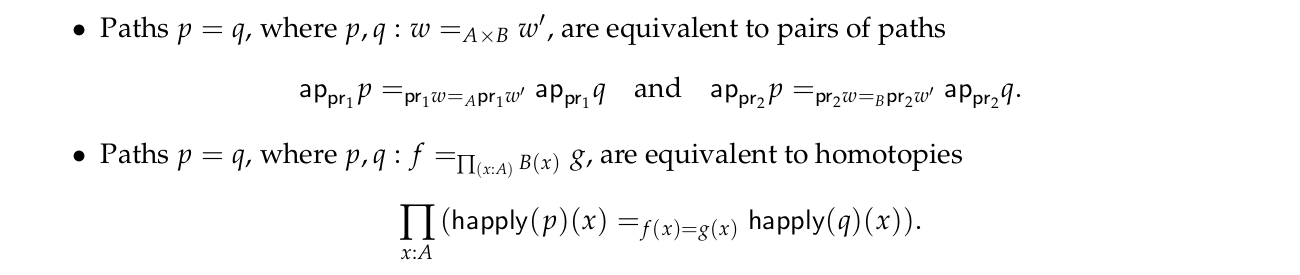
\includegraphics[scale=0.25]{2paths.png}
}}

\end{frame}

\begin{frame}{Ścieżki między ścieżkami 2 - interpretacja}
\begin{itemize}
	\item Z powyższego twierdzenia płyną daleko idące wnioski.
	\item Jeżeli mamy charakteryzację typu $A$ za pomocą równowazności $A \simeq B$, to mamy też charakteryzację ścieżek w $A$ (na dowolnym poziomie) za pomocą ścieżek w $B$.
	\item Jeżeli mamy charakteryzację ścieżek między punktami w $A$, to mamy charakteryzację dowolnych ścieżek w $A$.
	\item Tak więc ścieżki między ścieżkami między parami to pary ścieżek między ścieżkami między komponentami par.
	\item Ścieżki między ścieżkami między funkcjami to homotopie na $\happly$.
\end{itemize}
\end{frame}

\begin{frame}{Strukturalizm 1 - ścieżki między półgrupami}

\begin{block}{Półgrupa}
$\displaystyle \text{Semigroup} \defn \sum_{A : \U} \sum_{m : A \to A \to A} \prod_{x\ y\ z : A} m(x, m(y, z)) = m(m(x, y), z)$
\end{block}

\begin{itemize}
	\item Półgrupa to typ wraz z działaniem binarnym, które jest łączne.
	\item Z charakteryzacji ścieżek dla par zależnych, funkcji oraz z aksjomatu uniwalencji wynika, że typ ścieżek między półgrupami jest równoważny typowi równoważności na ich nośnikach, które zachowują działanie $m$.
	\item Tak więc ścieżka między półgrupami to homomorficzna równoważność, czyli, w klasycznym rozumieniu, izomorfizm półgrup.
\end{itemize}

\end{frame}

\begin{frame}{Strukturalizm 2 - filozofia w praktyce}
\begin{itemize}
	\item Strukturalizm to filozofia matematyki, która twierdzi, że teorie matematyczne opisują strukturę obiektów matematycznych.
	\item Strukturę obiektu można rozumieć jako związki łączące go z innymi obiektami.
	\item Wobec tego obiekty matematyczne nie posiadają żadnych wewnętrznych właściwości i są zdeterminowane przez swoją strukturę.
	\item W praktyce znaczy to na przykład, że ze strkturalistycznego punktu widzenia izomorficzne półgrupy są identyczne.
	\item HoTT świetnie realizuje filozoficzne założenia strukturalizmu - jak się przekonaliśmy, izomorficzne półgrupy faktycznie są równe, czyli połączone ścieżką w typie półgrup. 
\end{itemize}

\end{frame}

\section{HITy}

\subsection{Część 1}

\begin{frame}{Typy induktywne 1 - przypomnienie}
\begin{itemize}
	\item Typ induktywny to typ wygenerowany w sposób ``wolny'' przez kolekcję konstruktorów.
	\item Typ $\textbf{0}$ jest generowany przez brak konstruktorów.
	\item Typ $\textbf{1}$ jest generowany przez konstruktor $* : \textbf{1}$
	\item Typ $\textbf{2}$ jest generowany przez konstruktory $0_{\textbf{2}} : \textbf{2}$ oraz $1_{\textbf{2}} : \textbf{2}$.
	\item Typ $\mathbb{N}$ jest generowany przez konstruktory $0$ oraz $\text{succ} : \mathbb{N} \to \mathbb{N}$
	\item $\text{List}$ to parametryczna rodzina typów generowana przez konstruktory $\text{Nil} : \Pi A : \U. \text{List}(A)$ oraz $\text{Cons} : \Pi A : \U. A \to \text{List}(A) \to \text{List}(A)$
	\item $=$ to indeksowana rodzina typów generowana tak jak było napisane na wcześniejszych slajdach.
\end{itemize}
\end{frame}

\begin{frame}{Typy induktywne 2 - więcej przykładów}

Za pomocą typów induktywnych da się zdefiniować dużo różnych rzeczy. Ćwiczenie: spróbuj zdefiniować:
\begin{itemize}
	\item Rodzinę $\text{Tree}$ drzew trzymających elementy danego typu wyłącznie w liściach (drzewo może być puste).
	\item Rodzinę $\text{Sorted}$ taką, że $\text{Sorted}(R, l)$ ma element, gdy lista $l$ jest posortowana według relacji porządku $R$ i nie ma elementu w przeciwnym razie.
	\item Rodzinę $\text{Perm}$ taką, że $\text{Perm}(l_1, l_2)$ ma element, gdy $l_1$ jest permutacją $l_2$ i nie ma elementu, gdy $l_1$ nie jest permutacją $l_2$.
	\item Rodzinę $\text{FreeMon}$ taką, że typ $\text{FreeMon}(A)$ jest wolnym monoidem na typie $A$. Uwaga: podchwytliwe.
\end{itemize}
\end{frame}

\begin{frame}{Wyższe typy induktywne 1 - motywacja}

Typy induktywne nie są jednak wszechmocne. Niektórych rzeczy zdefiniować się nie da:
\begin{itemize}
	\item Nie da się zdefiniować typów ilorazowych, np. nie da się zdefiniować liczb wymiernych $\mathbb{Q}$ jako par $\mathbb{Z} \times \mathbb{Z}$ podzielonych przez relację równoważności $\sim$ zdefiniowaną jako $(a, b) \sim (a', b') \defn ab' = a'b$.
	\item Nie da się zdefiniować rodziny $\text{FreeGrp}$, która reprezentuje grupę wolną na danym typie.
	\item W ogólności, nie da się zdefiniować niczego, co wymaga utożsamienia ze sobą dwóch elementów danego typu. Wynika to z faktu, że konstruktory typów induktywnych są injektywne.
\end{itemize}
\end{frame}

\begin{frame}{Wyższe typy induktywne 2 - sposób}
\begin{itemize}
	\item Wyższe typy induktywne generalizują typy induktywne w następujący sposób.
	\item Pozwalamy sobie na to, że poza zwykłymi konstruktorami (które od teraz będziemy nazywać konstruktorami punktów) możemy robić też konstruktory ścieżek, które wkładają do typu nowe ścieżki.
	\item Ponieważ ścieżki to równość, możemy dzięki temu utożsamiać ze sobą różne punkty i w ten sposób zdefiniować rzeczy z powyższego slajdu.
	\item Ale otwierają się przed nami również inne możliwości: możemy bezpośrednio definiować przestrzenie topologiczne takie jak odcinek albo okrąg, wesołe konstrukcje logiczne takie jak $n$-trunkacja, która przekształca dany typ w $n$-typ, oraz rzeczy przydatne w teorii kategorii, np. kogranice.
\end{itemize}
\end{frame}

\begin{frame}{Wyższe typy induktywne 3 - filozofia}
\begin{itemize}
	\item Przypomnijmy, że w typach zdefiniowanych przez wyższą indukcję mogą być rzeczy, których tam nie włożyliśmy. Np. jeżeli wrzucimy do typu jakąś ścieżkę $p$, to pojawi się w nim także ścieżka $p^{-1}$.
	\item A priori nie wiadomo, jak się zachowują włożone przez nas ścieżki. Mogą one być trywialne albo i nie.
	\item Mimo, że możemy do typu dodawać ścieżki, to wciąż definiujemy pojedynczy typ - nie redefiniujemy typu $=$. Definiowany przez nas typ dostanie swoją własną regułę indukcji, a reguła indukcji po ścieżkach pozostanie taka jak była - nowe ścieżki nie mają na nią wpływu.
	\item Wymiar konstruktora ma nikły wpływ na strukturę ścieżek: jeżeli definiując $B$ dodamy konstruktor punktów typu $A \to B$, to wszystkie ścieżki z $A$ zostają wstrzyknięte do $B$.
\end{itemize}
\end{frame}

\subsection{Część 2}

\begin{frame}{Odcinek 1 - definicja}

\begin{center}
$\displaystyle
	\frac{}{\Gamma \vdash \I : \U}
$
\end{center}

\begin{center}
$\displaystyle
	\frac{}{\Gamma \vdash \IZ : \I}
$ \quad
$\displaystyle
	\frac{}{\Gamma \vdash \II : \I}
$ \quad
$\displaystyle
	\frac{}{\Gamma \vdash \seg : \IZ = \II}
$
\end{center}

\begin{center}
$\displaystyle
	\dfrac{\Gamma \vdash A   : \I \to \U			\quad
		  \Gamma \vdash a_0 : A(\IZ)			\quad
		  \Gamma \vdash a_1 : A(\II)			\quad
		  \Gamma \vdash p   : \seg_*(a_0) = a_1
		 }
		 {\Gamma \vdash \text{ind}_\I(A, a_0, a_1, p) : \Pi i : \I. A(i)}
$
\end{center}

\begin{center}
$\displaystyle
	\dfrac{\Gamma \vdash A   : \I \to \U			\quad
		  \Gamma \vdash a_0 : A(\IZ)			\quad
		  \Gamma \vdash a_1 : A(\II)			\quad
		  \Gamma \vdash p   : \seg_*(a_0) = a_1
		 }
		 {\Gamma \vdash \text{ind}_\I(A, a_0, a_1, p, \IZ) \equiv a_0 : A(\IZ)}
$
\end{center}

\begin{center}
$\displaystyle
	\dfrac{\Gamma \vdash A   : \I \to \U			\quad
		  \Gamma \vdash a_0 : A(\IZ)			\quad
		  \Gamma \vdash a_1 : A(\II)			\quad
		  \Gamma \vdash p   : \seg_*(a_0) = a_1
		 }
		 {\Gamma \vdash \text{ind}_\I(A, a_0, a_1, p, \II) \equiv a_1 : A(\II)}
$
\end{center}

\begin{center}
$\displaystyle
	\dfrac{\Gamma \vdash A   : \I \to \U			\quad
		  \Gamma \vdash a_0 : A(\IZ)			\quad
		  \Gamma \vdash a_1 : A(\II)			\quad
		  \Gamma \vdash p   : \seg_*(a_0) = a_1
		 }
		 {\Gamma \vdash \text{wut} : \apd{\text{ind}_\I(A, a_0, a_1, p)}{\seg} = p}
$
\end{center}

\end{frame}

\begin{frame}{Odcinek 2 - uwagi}
\begin{itemize}
	\item Dla wyższych typów tak jak i dla zwykłych mamy 5 rodzajów reguł.
	\item Reguły formacji i eliminacji pozostają bez zmian.
	\item Reguły wprowadzania mogą robić ścieżki między punktami definiowanego typu.
	\item Reguły obliczania dla punktów również nie ulegają zmianom. Musimy jednak zadbać o to, żeby napisać reguły obliczania dla ścieżek. Robimy to za pomocą funkcji $\text{ap}$ (dla rekursora) i $\text{apd}$ (dla reguły indukcji). Ponieważ $\text{apd}$ został zdefiniowany wewnątrz naszej teorii, a reguły żyją na metapoziomie, to reguły obliczania dla ścieżek nie są definicyjne (tzn. $\equiv$), tylko same są ścieżkami i wobec tego musimy je jakoś nazwać.
	\item Wobec tego definiując za pomocą równań i dopasowania do wzorca w przypadku ścieżek będziemy używać hybrydowej notacji $:=$
\end{itemize}
\end{frame}

\begin{frame}{Odcinek 3 - o co tak naprawdę chodzi w indukcji}
\begin{itemize}
	\item Jeżeli reguła eliminacji dla odcinka wydaje ci się mistyczna, to posłuchaj poniższej bajki na temat indukcji.
	\item Każdy typ induktywny ma pewną strukturę. W przypadku odcinka są to punkty $\IZ$ i $\II$ wraz z łączącą je ścieżką $\seg$.
	\item Rekursor (czyli upośledzona reguła eliminacji) mówi, że jeżeli znajdziemy w jakimś typie taką samą strukturę (dwa punkty $a_0$ i $a_1$ połączone ścieżką $p$), to możemy zrobić funkcję $f$, która spełnia $f(\IZ) \defn a_0, f(\II) \defn a_1, \ap{f}{\seg} := p$.
	\item Reguła eliminacji z poprzedniego slajdu jest uogólnieniem powyższego opisu na typy zależne.
\end{itemize}
\end{frame}

\begin{frame}{Odcinek 4 - właściwości}
	
\begin{block}{6.3.1 Odcinek jest ściągalny}
$\isContr(\I)$
\end{block}

\begin{block}{6.3.2 Odcinek implikuje ekstensjonalność}
Niech $f, g : A \to B$ będą funkcjami i niech $H : \Pi x : A. f(x) = g(x)$ będzie homotopią. Wtedy $f = g$ bez używania aksjomatu ekstensjonalności.
\end{block}

\end{frame}

\begin{frame}{Odcinek 5 - dowód lematu 6.3.2}
\begin{block}{Dowód lematu 6.3.2}
	Przez rekursję po odcinku definiujemy nastepującą funkcję: \\
	$p : A \to \I \to B$ \\
	$p(x, \IZ) \defn f(x)$ \\
	$p(x, \II) \defn g(x)$ \\
	$\ap{p(x)}{\seg} := H(x)$ \\~\
	
	Teraz definiujemy \\
	$q : \I \to (A \to B)$ \\
	$q(i) \defn \lambda x : A. p(x, i)$ \\~\
	
	Mamy $q(\IZ) \equiv \lambda x : A. p(x, \IZ) \equiv \lambda x : A. f(x) \equiv f$ i analogicznie $q(\II) \equiv g$, a zatem $\ap{q}{\seg} : f = g$
\end{block}
\end{frame}


\begin{frame}{Okrąg 1 - definicja}

\makebox[\linewidth]{\parbox{12cm}
{
	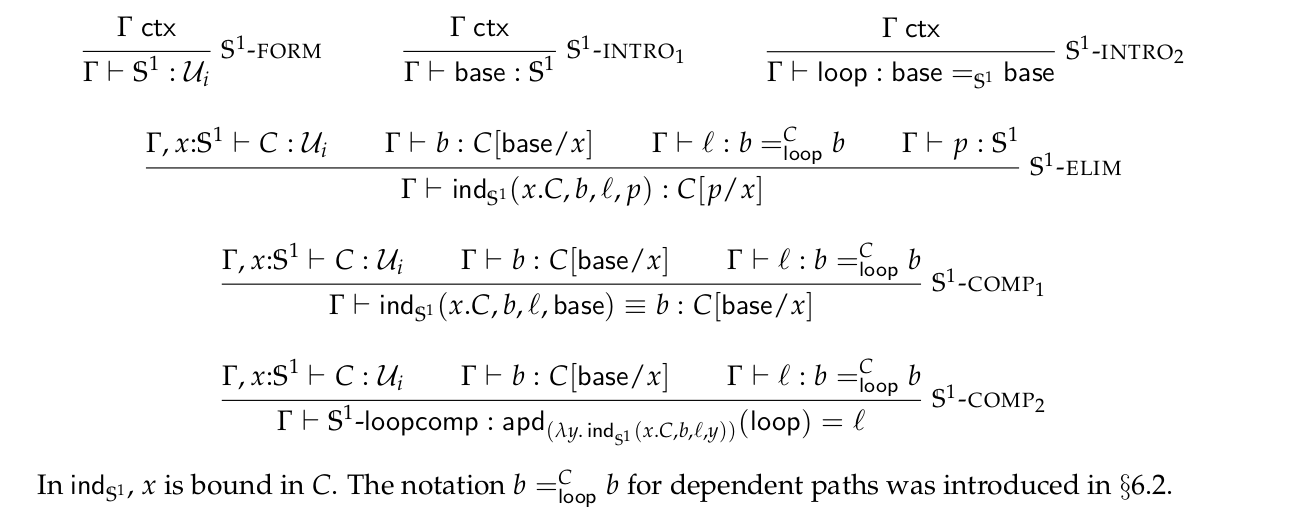
\includegraphics[scale=0.25]{circle.png}
}}

Ćwiczenie: opisz rekursor dla okręgu w taki sposób, jaki opisany został rekursor dla odcinka.

\end{frame}

\begin{frame}{Okrąg 2 - właściwości}
	
\begin{block}{6.2.9 Okrąg to faktycznie okrąg}
$(\hS \to A) \simeq \sum_{x : A} x = x$
\end{block}

\begin{block}{Lemat 6.4.1}
$\looop \neq \refl{\base}$
\end{block}

\begin{block}{Dowód lematu 6.4.1}
Załóżmy, że $\looop = \refl{\base}$. Weźmy dowolny typ $A$ z punktem $x : A$ i pętlą $p : x = x$ (są takie). Wtedy na mocy rekursora dla $\hS$ możemy zdefiniować funkcję $f : \hS \to A$ następująco: \\

$f(\base) \defn x$ \\
$\ap{f}{\looop} := p$ \\

Mamy stąd $p = \ap{f}{\looop} = \ap{f}{\refl{\base}} = \refl{f(\base)} = \refl{x}$. Wobec tego każdy typ mający choć jeden punkt jest zbiorem, co jest sprzeczne (bo np. uniwersum nie jest zbiorem).
\end{block}

\end{frame}

\section{$n$-typy}

\subsection{Część 1}

\begin{frame}{Klasyfikacja typów}
\begin{itemize}
	\item W HoTT poza punktami mamy też różne mniej lub bardziej skomplikowane ścieżki.
	\item Wobec tego mądrym pomysłem wydaje się klasyfikowanie typów ze względu na złożoność ścieżek, jakie w nich występują.
	\item $n$-typ, to (w przybliżeniu) typ, w którym wszystkie ścieżki powyżej $n$-tego poziomu są trywialne. $n$-typy bywają też nazywane typami $n$-obciętymi (ang. $n$-truncated).
	\item Dualnym pojęciem jest pojęcie $n$-spójności (ang. $n$-connectedness). Typ $n$-spójny to taki, w którym wszystkie ścieżki poniżej $n$-tego poziomu są trywialne.
	\item My zajmiemy się tylko typami $n$-obciętymi. Zanim jednak omówimy je w ogólności, zobaczmy kilka pierwszych poziomów.
\end{itemize}
\end{frame}

\begin{frame}{Ściągalność 1 - definicja i właściwości}

\begin{block}{Ściągalność}
$
\displaystyle
\isContr(A) \defn \sum_{c : A} \prod_{x : A} c = x
$
\end{block}

Typ jest ściągalny gdy ma punkt centralny, który jest połączony ścieżką z każdym innym punktem tego typu. Nazwa bierze się stąd, że możemy wszystkie punkty ściągnąć do centrum. Wobec tego typ ściągalny jest równoważny typowi $\textbf{1}$.

\end{frame}

\begin{frame}{Ściągalność 2 - filozofowanie}
\begin{itemize}
	\item Mogłoby się wydawać, że ściągalność jest nieciekawa, skoro typy ściągalne są równoważne (czyli równe, dzięki uniwalencji) typowi $\textbf{1}$.
	\item Kluczowy jest jednak fakt, że typy, które same w sobie są wysoce nietrywialne i z pewnością nie są ściągalne, złożone do kupy mogą dać typ, który jest ściągalny.
	\item Jest tak dlatego, że wzajemne zależności między obiektami mogą wykluczyć wszystkie kombinacje poza jedną.
	\item Najprostszym przykładem tego rodzaju jest sparowanie jakiegoś obiektu ze specyfikacją, która charakterzyuje go w sposób unikalny.
	\item Co ważne, nawet jeżeli typ jest ściągalny, to zachowuje swoje właściwości obliczeniowe.
\end{itemize}
\end{frame}

\begin{frame}{Ściągalność 3 - przykłady}
\begin{itemize}
	\item Oczywiście $\textbf{1}$ jest ściągalny.
	\item Odcinek $\I$ jest ściągalny. Mimo tego, jak widzieliśmy, może on posłużyć nam do udowodnienia aksjomatu ekstensjonalności.
	\item Ściągalny jest typ funkcji sortujących. Mimo, że funkcji między listami jest dużo, to dobrze wyrażona specyfikacja sortowania unikalnie charateryzuje jedyną słuszną funkcję sortującą.
	\item Dla dowolnego $a : A$ typ $\sum_{x : A} a = x$ jest ściągalny i dlatego właśnie indukcja po ścieżkach (w wersji based) działa.
	\item Podobnie ściągalny jest typ $\sum_{x,y : A} x = y$ i dlatego właśnie indukcja po ścieżkach (w wersji unbased) działa.
\end{itemize}
\end{frame}

\begin{frame}{Zdania}

\begin{block}{Zdanie}
$\isProp(A) \defn \prod_{x, y : A} x = y$ \\
$\Prop \defn \sum_{A : \U} \isProp(A)$
\end{block}

\begin{itemize}
	\item Zdanie to typ, który może mieć co najwyżej jeden punkt. Przypomina to tradycyjną logikę: twierdzenie (zdanie) może mieć dowód albo nie.
	\item $\textbf{0}$ i $\textbf{1}$ są zdaniami. Odpowiadają one fałszowi i prawdzie.
	\item Dla każdego $A : \U$ typ $\neg A \defn A \to \textbf{0}$ jest zdaniem.
	\item Typ $\isequiv(f)$ jest zdaniem, ale typ $\qinv(f)$ może NIE być zdaniem i dlatego właśnie mieliśmy problem.
	\item O ile wszystkie zdania fałszywe są równe i podobnie wszystkie zdania prawdziwe są równe, to $\Prop$ nie jest tym samym co $\textbf{2}$, gdyż w ogólności nie jesteśmy w stanie rozstrzygnąć, czy mamy do czynienia ze zdaniem prawdziwym, czy fałszywym.
\end{itemize}

\end{frame}

\subsection{Część 2}

\begin{frame}{Zbiory}

\begin{block}{Zbiór}
$\isSet(A) \defn \prod_{x, y : A} \prod_{p, q : x = y} p = q$ \\
$\Set \defn \sum_{A : \U} isSet(A)$
\end{block}

\begin{itemize}
	\item Intuicyjnie: zbiór to typ, w którym może być dużo punktów, ale nie są one połączone ścieżkami (tzn. wszystkie ścieżki są trywialne).
	\item Każde zdanie jest zbiorem, więc w szczególności $\textbf{0}$ i $\textbf{1}$.
	\item Na mocy naszej charakteryzacji typ $\textbf{2}$ jest zbiorem.
	\item Typ $\mathbb{N}$ jest zbiorem (ćwiczenie: udowodnij za pomocą metody encode-decode).
	\item Wszystko, co jesteśmy w stanie zdefiniować za pomocą zwykłych typów induktywnych jest zbiorem, pod warunkiem że jako argumenty konstruktorów również bierze zbiory.
\end{itemize}

\end{frame}

\begin{frame}{Grupoidy}

\begin{block}{Grupoid}
$\isGrpd(A) \defn \prod_{x, y : A} \prod_{p, q : x = y} \prod_{r, s : p = q} r = s$ \\
$\Grpd \defn \sum_{A : \U} \isGrpd(A)$
\end{block}

\begin{itemize}
	\item Grupoid to typ, który może mieć punkty i ścieżki między punktami, ale nie może mieć ścieżek między ścieżkami.
	\item Okrąg $\hS$ jest grupoidem - widzieliśmy, że pętla $\looop$ nie jest trywialna.
	\item Uniwersum wszystkich zbiorów $\Set$ jest grupoidem, ponieważ typ $\textbf{2}$ ma nietrywialną pętlę, zrobioną z negacji boolowskiej za pomocą aksjomatu uniwalencji. Nie jest ona trywialna, bo negacja nie jest identycznością.
\end{itemize}

\end{frame}

\begin{frame}{$n$-typy 1 - definicja}

Na mocy pewnych zaszłości historycznych numerowanie $n$-typów zaczyna się od $-2$, a nie od $0$.

\begin{block}{$n$-typ}
$\text{is-}(-2)\text{-Type}(A) \defn \sum_{c : A} \prod_{x : A} c = x$ \\
$\text{is-}(n + 1)\text{-Type}(A) \defn \prod_{x, y : A} \text{is-}n\text{-Type}(x = y)$ \\
$n\text{-Type} \defn \sum_{A : \U} \text{is-}n\text{-Type}(A)$
\end{block}

Widać, że:
\begin{itemize}
	\item $-2$-typy to typy ściągalne.
	\item $-1$-typy to zdania.
	\item $0$-typy to zbiory.
	\item $1$-typy to grupoidy.
\end{itemize}

\end{frame}

\begin{frame}{$n$-typy 2 - właściwości}
\begin{itemize}
	\item Jeżeli $A$ jest $n$-typem, to jest też $(n + 1)$-typem. Intuicyjnie: skoro $A$ ma trywialną strukturę powyżej poziomu $n$, to ma też trywialną strukturę powyżej poziomu $(n + 1)$
	\item Jeżeli $A : \U$ jest $n$-typem i $B : A \to \U$ jest rodziną $n$-typów, to $\sum_{x : A} B(x)$ oraz $\prod_{x : A} B(x)$ także są $n$-typami.
	\item W szczególności jeżeli $A$ i $B$ są $n$-typami, to $A \times B$ oraz $A \to B$ także są $n$-typami.
	\item Jeżeli $A$ i $B$ są $n$-typami dla $n \geq 0$, to $A + B$ jest $n$-typem.
	\item Uwaga: jeżeli $A$ i $B$ są $-2$-typami, to $A + B$ jest $0$-typem. Podobnie jeżeli $A$ i $B$ są $-1$-typami, to $A + B$ może być $-2$-typem, $-1$-typem lub $0$-typem.
	\item Typ $\text{is-}n\text{-Type}$ jest zdaniem.
\end{itemize}
\end{frame}

\begin{frame}{$n$-typy 3 - (kontr)przykłady}
\begin{itemize}
	\item Typ $\textbf{1}$ jest $n$-typem dla każdego $n$.
	\item Typ $n\text{-Type}$ jest $(n + 1)$-typem.
	\item Jednak ważniejsze jest to, jakie typy nie są $n$-typami.
	\item $n$-te uniwersum $\U_n$ nie jest $n$-typem.
	\item W klasycznej teorii homotopii $k$-wymiarowa (hiper)sfera $\mathbb{S}^k$ nie jest $n$-typem dla żadnego $k \geq 2$. W HoTTBooku nie ma na to dowodu.
	\item Jeżeli powyższe jest prawdą, to żadne uniwersum nie jest $n$-typem, bo zawiera hipersferę.
	\item Konkretny (kontr)przykład (8.8.6): Niech $A \defn \prod_{n : \mathbb{N}} B(n)$, gdzie $B : \mathbb{N} \to \U$ jest taką rodziną typów, że typ $B(n)$ zawiera $n$-pętlę, która nie jest równa trywialnej $n$-pętli. Wtedy $A$ nie jest $n$-typem dla żadnego $n : \mathbb{N}$.
\end{itemize}
\end{frame}

\section{Logika}

\subsection{Część 1}

\begin{frame}{Logika}
\begin{itemize}
	\item Poznawszy wszystkie trzy filary HoTT rzućmy na koniec okiem na konsekwencje, jakie niosą one dla logiki.
	\item W teorii typów częstym sloganem jest ``propositions as types'', który pozwala nam kodować zdania jako typy.
	\item Wiemy już jednak, że nasze typy reprezentują $\omega$-grupoidy (czyli przestrzenie). Poznaliśmy też typ zdań $\Prop$ - są to przestrzenie mogące mieć co najwyżej jeden punkt.
	\item Spróbujmy jakoś uporządkować ten konceptualny bałagan.
\end{itemize}
\end{frame}

\begin{frame}{Logika klasyczna 1 - problem}

Większość matematyki jest robiona klasycznie, mimo że jest to niegodziwe. Wobec tego my też chcielibyśmy w ostateczności móc zrobić trochę klasycznej matematyki. Sprawy się jednak komplikują.

\begin{block}{3.2.2 Prawo podwójnej negacji nie zachodzi dla dowolnych typów}
$\neg \prod_{A : \U} \neg\neg A \to A$
\end{block}

\begin{block}{3.2.7 Prawo wyłączonego środka nie zachodzi dla dowolnych typów}
$\neg \prod_{A : \U} A + \neg A$
\end{block}

\begin{block}{Moje uogólnienie lematu 3.2.2}
Niech $F : \U \to \Prop$ i niech $x : F(\textbf{2})$. Wtedy \\~\

$\neg \prod_{A : \U} F(A) \to A$
\end{block}

\end{frame}

\begin{frame}{Logika klasyczna 2 - interpretacja}
\begin{itemize}
	\item Dowód lematu 3.2.2 jest dość techniczny. Ciężko go zobrazować.
	\item Typ $\neg\neg A$ możemy zinterpretować jako typ $A$, z którego wyrzucono wszystko poza jednym punktem, o ile były w nim jakieś punkty.
	\item Wobec tego typ $\neg\neg A \to A$ możemy zinterpretować jako operację odzyskującą z tak obciętego typu jakiś punkt.
	\item Można tę operację wykonać dla każdego typu z osobna, ale nie można tego zrobić w taki sam sposób dla wszystkich typów.
	\item Uogólnienie lematu pokazuje, że problemem faktycznie nie jest podwójna negacja, ale utrata informacji związana z obcięciem przestrzeni.
	\item Jeżeli przyjrzeć się dowodowi z książki, to ostateczna konkluzja brzmi: (naiwne) prawo wyłączonego środka jest sprzeczne z aksjomatem uniwalencji.
\end{itemize}
\end{frame}

\begin{frame}{Logika klasyczna 3 - rozwiązanie}

Tak więc możemy skonkludować, że nasze przestrzenie (czyli dowolne typy) zawierają za dużo informacji, żeby robić na nich logikę. Dla zdań (czyli typów z uniwersum $\Prop$) problem znika.

\begin{block}{Prawo podwójnej negacji}
$\text{DNE} \defn \prod_{P : \Prop} \neg\neg P \to P$
\end{block}

\begin{block}{Prawo wyłączonego środka}
$\text{LEM} \defn \prod_{P : \Prop} P + \neg P$
\end{block}

Powyższe definicje pokazują, jak wyglądają poprawnie sformułowane prawo podwójnej negacji oraz prawo wyłączoengo środka stosujące się jedynie do zdań. Tak sformułowane aksjomaty możemy przyjąć bez popadania w sprzeczność.

\end{frame}

\begin{frame}{Trunkacja 1 - motywacja}
\begin{itemize}
	\item Okazało się, że nasze typy zawierają za dużo informacji, aby móc służyć jako zdania. Tylko niektóre z nich się do tego nadają.
	\item Jednak to nie koniec problemów - nasze spójniki też nie są idealne. W tradycyjnej logice spójniki przekształcają zdania w zdania, u nas natomiast tak nie jest: suma dwóch zdań nie musi być zdaniem, np. $\textbf{1} + \textbf{1} = \textbf{2}$.
	\item Jeszcze hardkorowiej sprawa ma się z sumą zależną: nawet jeżeli dla każdego $x : A$ typ $B(x)$ jest zdaniem, to typ $\sum_{A : \U} B(x)$ może być dowolnie skomplikowaną przestrzenią (bo $A$ może być dowolnie skomplikowaną przestrzenią).
	\item Jak widać, nasze spójniki $+$ oraz $\sum$ są zbyt konstruktywne. Spróbujmy zatem wynaleźć takie, które zachowywałyby właściwość bycia zdaniem.
\end{itemize}
\end{frame}

\begin{frame}{Trunkacja 2 - pomysł}
\begin{itemize}
	\item Pomysł jest prosty. Widzieliśmy już, że za pomocą wyższych typów induktywnych możemy dodawać do typów dowolne ścieżki.
	\item Wobec tego moglibyśmy zdefiniować spójnik $\lor$ podobnie do $+$, ale wrzucić do niego tyle ścieżek, żeby jego wynik był zdaniem.
	\item Będziemy jednak sprytniejsi i zdefiniujemy trunkację zdaniową (ang. propositional truncation) - operację, która zamienia każdy typ w zdanie.
\end{itemize}
\end{frame}

\begin{frame}{Trunkacja 3 - definicja}

\begin{center}
$\displaystyle
	\frac{\Gamma \vdash A : \U}{\Gamma \vdash \trf{A} : \U}
$
\end{center}

\begin{center}
$\displaystyle
	\frac{\Gamma \vdash x : A}{\Gamma \vdash \tri{x} : \trf{A}}
$ \quad
$\displaystyle
	\frac{\Gamma \vdash A : \U	\quad
		  \Gamma \vdash x : A	\quad
		  \Gamma \vdash y : A	\quad
		 }
		 {\Gamma \vdash \text{wut} : x = y}
$
\end{center}

\begin{center}
$\displaystyle
	\frac{\Gamma \vdash A : \U		\quad
		  \Gamma \vdash B : \Prop	\quad
		  \Gamma \vdash f : A \to B
		 }
		 {\Gamma \vdash \text{ind}_{\trf{A}} : \trf{A} \to B}
$
\end{center}

\begin{center}
$\displaystyle
\frac{\Gamma \vdash A : \U		\quad
	  \Gamma \vdash B : \Prop	\quad
	  \Gamma \vdash f : A \to B	\quad
	  \Gamma \vdash x : A
	 }
	 {\Gamma \vdash \text{ind}_{\trf{A}}(\tri{x}) \equiv f(x) : \trf{A}}
$
\end{center}

\end{frame}

\begin{frame}{Trunkacja 4 - interpretacja}
\begin{itemize}
	\item Reguła wprowadzania $\tri{-}$ wstrzykuje punkty $A$ do $\trf{A}$.
	\item Reguła wprowadzania $\text{wut}$ sprawia, że wszystkie tak wstrzyknięte punkty są połączone ścieżkami każdy z każdym.
	\item Reguła eliminacji mówi nam, że jeżeli $A$ implikuje zdanie $B$, to zdanie $B$ wynika już z obciętego $A$.
	\item Reguła obliczania to tylko formalność.
\end{itemize}
\end{frame}

\subsection{Część 2}

\begin{frame}{Logika zdań 1 - definicje}

\makebox[\linewidth]{\parbox{10.5cm}
{
	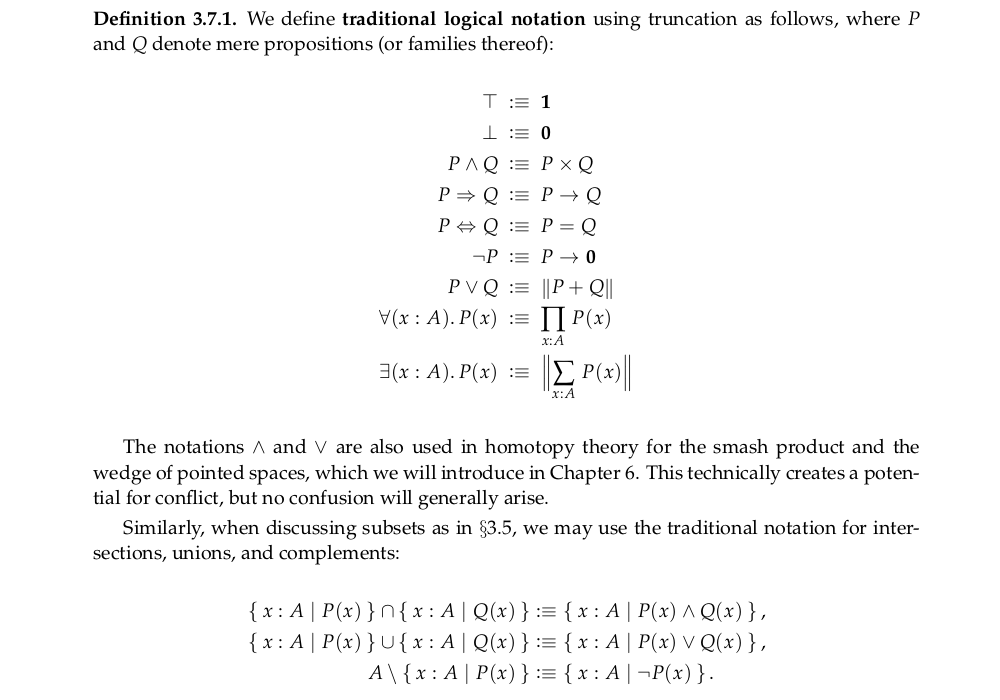
\includegraphics[scale=0.3]{logic.png}
}}
	
\end{frame}

\begin{frame}{Logika zdań 2 - interpretacja}
\begin{itemize}
	\item Dysjunkcję definiujemy jako obciętą sumę rozłączną, zaś kwatyfikator egzystencjalny jako obciętą parę zależną. Tym sposobem uzyskujemy spójniki, za pomocą których możemy rozumować tak jak dotychczas, ale tylko gdy dowodzimy zdań.
	\item Gdy konstruujemy jakieś obiekty, nie możemy pozbyć się trunkacji, a więc nie możemy uzależnić naszych konstrukcji od wyboru lewego lub prawego dysjunktu ani od konkretnego punktu występującego w sumie zależnej. Dzięki temu wiemy, że dysjunkcja jest prawdziwa, ale nie wiemy, który dysjunkt jej dowodzi. Podobnie wiemy, że istnieje punkt spełniający warunek, ale nie wiemy, jaki to punkt.
	\item Zauważmy też, że dla zdań $P$ i $Q$ jeżeli $P \to Q$ oraz $Q \to P$, to $P \simeq Q$, a więc także $P = Q$. Aksjomat uniwalencji w przypadku zdań mówi nam, że ścieżki między zdaniami reprezentują równoważność logiczną.
	\item Pozostałe spójniki zachowują właściwość bycia zdaniem.
\end{itemize}
\end{frame}

\begin{frame}{Zasada unikalnego wyboru 1 - rozważania}
\begin{itemize}
	\item Może się wydawać, że nasza logika jest trochę upośledzona - brak możliwości rozłożenia sumy (rozłącznej/zależnej) na przypadki podczas konstrukcji może zniechęcać do ich używania.
	\item Jest jednak pewna sprytna technika, która pozwala obejść to ograniczenie.
	\item Prezentuje się ona zazwyczaj tak: chcąc z $\trf{A}$ skonstruować $B$, które może nie być zdaniem, robimy predykat $P : B \to \U$, taki, że typ $\sum_{x : B} P(x)$ jest ściągalny. Wtedy przy konstruowaniu funkcji $\trf{A} \to \sum_{x : B} P(x)$ możemy pozbyć się trunkacji.
	\item Po więcej zobacz rozdział 3.9 w HoTTBooku.
\end{itemize}
\end{frame}

\begin{frame}{Zasada unikalnego wyboru 2 - przykład}
	
\begin{block}{Zadanie 3.19 i 3.23}
Niech $P : \mathbb{N} \to \U$ będzie rodziną typów. Wtedy \\~\

\begin{center}
$\displaystyle \left|\left|\sum_{n : \mathbb{N}} P(n)\right|\right| \to \sum_{n : \mathbb{N}} P(n)$
\end{center}
\end{block}

\begin{block}{Dowód}
Wiemy, że istnieje jakieś $n$ spełniające $P$, ale nie wiemy jakie, więc nie możemy go rozpakować. Zamiast konstruować dowolne $n$ spełniające $P$, możemy jednak skonstruować najmniejsze takie $n$, tzn. element typu $\sum_{n : \mathbb{N}} P(n) \times \prod_{m : \mathbb{N}} P(m) \to n \leq m$. Jest ono unikalne, a zatem cały ten typ jest zdaniem. Możemy teraz odpakować $n$ z przesłanki i zrobić przeszukiwanie od $n$ do $0$ w poszukiwaniu minimalnego $n$.
\end{block}

\end{frame}

\begin{frame}{Aksjomat wyboru 1 - problem}

Moglibyśmy pokusić się o sformułowanie Aksjomatu Wyboru w następujący sposób.

\begin{block}{Aksjomat ``Wyboru'', który tak naprawdę nic nie wybiera}
Dla typu $A : \U$, rodziny typów $B : A \to \U$ oraz rodziny typów $R : \prod_{x : A} B(x) \to \U$ zachodzi: \\~\

$\displaystyle
	\left(\prod_{x : A} \sum_{y : B(x)} R(x, y)\right) \to
	\sum_{f : \Pi x : A. B(x)} \prod_{x : A} R(x, f(x))
$
\end{block}

Niestety ten sposób jest upośledzony, gdyż nie jest to aksjomat, tylko twierdzenie, i to bardzo proste do udowodnienia. Mankament ten wynika z faktu, że wszystkie wybory zostały już dokonane - nasza interpretacja sumy zależnej sprawia, że żeby uzyskać konkluzję, wystarczy odopwiednio przepakować przesłankę. Ten Aksjomat ``Wyboru'' jest zupełnie jak wybory w Polsce.

\end{frame}

\begin{frame}{Aksjomat wyboru 2 - trunkacja na ratunek}

Jak nietrudno się domyślić, nasz problem możemy rozwiązać wciskają gdzie trzeba trunkację.

\begin{block}{Jedyny słuszny Aksjomat Wyboru w pełnej krasie}
Dla zbioru $A : \Set$, rodziny zbiorów $B : A \to \Set$ oraz relacji (czyli rodziny zdań) $R : \prod_{x : A} B(x) \to \Prop$ zachodzi: \\~\

$\displaystyle
	\left(\prod_{x : A} \left|\left|\sum_{y : B(x)} R(x, y)\right|\right|\right) \to
	\left|\left|\sum_{f : \Pi x : A. B(x)} \prod_{x : A} R(x, f(x))\right|\right|
$ \\~\

W naszej nowej notacji logicznej możemy to zapisać tak: \\~\

$\displaystyle
	(\forall x : A. \exists y : B(x). R(x, y)) \implies
$ \\
$\displaystyle \qquad
	\exists f : (\Pi x : A. B(x)). \forall x : A. R(x, f(x))
$
\end{block}

\end{frame}

\begin{frame}{Aksjomat wyboru 3 - interpretacja}
\begin{itemize}
	\item Dzięki zastosowaniu trunkacji w przesłance wiemy, że dla $x : A$ istnieje jakieś $y : B(x)$, ale nie wiemy jakie. To sprawia, że żaden wybór nie został jeszcze dokonany.
	\item Podobnie dzięki zastosowaniu trunkacji w konkluzji aksjomat mówi, że istnieje jakaś funkcja, ale nie wiadomo jaka. To sprawia, że żaden wybór nie został z góry dokonany.
	\item Składając to do kupy widzimy, że tym razem Aksjomat Wyboru faktycznie coś wybiera.
	\item Jednak to nie wszystko. Zwróć uwage, że ten aksjomat dotyczy jedynie zbiorów, rodzin zbiorów oraz relacji, w przeciwieństwie do poprzedniego, który dotyczył typów i rodzin typów.
	\item Powód tego jest prosty (ale skomplikowany).
\end{itemize}
\end{frame}

\begin{frame}{Aksjomat wyboru 4 - zaskoczenie}

\begin{block}{Lemat 3.8.5}
Istnieje taki typ $A$ i rodzina zbiorów $B : A \to \U$, że Aksjomat Wyboru nie zachodzi.
\end{block}

Dowód jest dość skomplikowany - po więcej zajrzyj do książki. \\~\

W telefgraficznym skrócie: wszystkiemu winne są nietrywialne ścieżki. Nie możemy beztrosko wybierać punktów, nie zwracając na nie uwagi. Tak jak remedium w przypadku prawa wyłączonego środka było ograniczenie się do zdań, tak w przypadku Aksjomatu Wyboru jest nim ograniczenie się do zbiorów.

\end{frame}

\section{Koniec}

\begin{frame}{Ostateczne wątpliwości}
\begin{itemize}
	\item W ramach ostatecznych wątpliwości mogą nam się nasunąć różne pytania.
	\item A co jeżeli Aksjomat Uniwalencji jest sprzeczny? Otóż nie jest. A jeżeli nie jest konstruktywny? Otóż jest. Świadkiem nam Kubiczna Teoria Typów. Jest to teoria typów, w której można programować za pomocą $n$-wymiarowych sześcianów: \url{https://ncatlab.org/nlab/show/cubical+type+theory}
	\item Jaka jest ogólna składnia/schemat definiowania wyższych typów induktywnych? Co wolno a czego nie? Otóż nie do końca wiadomo, choć czynione są postępy: \url{http://drops.dagstuhl.de/opus/volltexte/2018/9190/}
	\item Jaka jest semantyka wyższych typów induktywnych? Jakaś jest: \url{https://arxiv.org/abs/1705.07088}, ale za dużo nie wiadomo.
	\item Będzie z tej mąki chleb? Tak.
\end{itemize}
\end{frame}

\begin{frame}{Podsumowanie}

HoTT daje nam:
\begin{itemize}
	\item Wyobraźnię w postaci interpretacji homotopicznej.
	\item Aksjomat Uniwalencji łatający filozoficzny smród i dający fajne sposoby rozumowania.
	\item Wyższe typy induktywne, które dają nam możliwość konstruktywnego rozwiązania masy problemów.
	\item Znacznie precyzyjniejszą analizę logiki, zarówno klasycznej jak i konstruktywnej.
	\item Możliwość formalizowania matematyki z prawdziwego zdarzenia, w tym teorii homotopii za pomocą metod syntetycznych.
	\item ... i wiele więcej.
\end{itemize}

\end{frame}

\begin{frame}{Żart 1}

Co łączy samobójcę, programistę imperatywnego, autobusiarza i homotopicznoteoriotypowca?

\end{frame}

\begin{frame}{Żart 2}

Lubią pętle.

\end{frame}

\begin{frame}{Zadania}

Zadanie 1: wykonaj wszystkie rzeczy oznaczone na slajdach jako ćwiczenie (poza ostatnią). \\~\

Zadanie 2: wykonaj ostatnią rzecz oznaczoną na slajdach jako ćwiczenie.

\end{frame}

\begin{frame}{Bibliografia 1}
\begin{itemize}
	\item Podstawowym źródłem wiedzy jest książka \url{https://homotopytypetheory.org/book/}, zwana potocznie HoTTBookiem.
	\item Jakaś prezentacja: \url{http://www.cs.nott.ac.uk/~psztxa/talks/edinburgh-13.pdf}
	\item Przyjazne przykłady wyższych typów induktywnych dla programistów: \url{http://www.cs.ru.nl/~herman/PUBS/HIT-programming.pdf}
\end{itemize}
\end{frame}

\begin{frame}{Bibliografia 2}
\begin{itemize}
	\item Filozoficzne rozważania na temat HoTT jako podstaw matematyki: \url{https://www.researchgate.net/publication/280671356_Does_Homotopy_Type_Theory_Provide_a_Foundation_for_Mathematics}
	\item Praca o podobnej tematyce: \url{https://arxiv.org/pdf/1601.05035.pdf}
	\item Ciekawa praca zachaczająca o filozofię matematyki, prezentująca coś, co można by nazwać pluralizmem topologicznym: \url{https://arxiv.org/abs/1703.03007}
\end{itemize}
\end{frame}

\end{document}